\documentclass[a4paper,oneside, english]{Tptesi2}

\usepackage[english]{babel}
\usepackage{listings}
\usepackage{amsmath,amssymb}
\usepackage{verbatim}
\usepackage{indentfirst}
\usepackage[utf8]{inputenc}
\usepackage{subfigure}
\usepackage{algorithmic}
\usepackage{framed}
\usepackage{rotating}
\usepackage{cite}
\usepackage{enumitem}
\usepackage{longtable}
\usepackage{booktabs}
\usepackage{graphicx} 
\usepackage{tabularx}
\usepackage[export]{adjustbox}

\usepackage{tikz}
\usepackage{rotating}

\usepackage{csquotes} % virgolette tipografiche per citazioni brevi
\usepackage{hyperref} % Per la gestione degli URL
\usepackage{xurl}     % Per la suddivisione degli URL lunghi


% FOOT NOTE
\usepackage{setspace}
\usepackage{footmisc}
\setstretch{0.9} 
\renewcommand{\footnotelayout} {\setstretch{0.9}} % Footnote con interlinia minore
\setlength{\skip\footins}{20pt} % Più spazio tra note e testo

% BOXES
\usepackage{tcolorbox}
\usepackage{capt-of}
\tcbuselibrary{theorems,breakable}
\newcounter{promptboxcounter}
\renewcommand{\thepromptboxcounter}{\arabic{promptboxcounter}}

\tcbset{
  promptboxstyle/.style={
    colback=gray!15,   
    colframe=gray!50, 
    boxrule=0.5pt,    
    arc=3pt,
    left=6pt, right=6pt, top=6pt, bottom=6pt,
    breakable,
    after skip=1.5pt, 
  }
}

\newtcolorbox{promptboxcontent}[1][]{%
  promptboxstyle,    
  #1               
}

\newcommand{\promptcaption}[2]{
  \refstepcounter{promptboxcounter}
  \par\vspace{4pt}
  \noindent \small Prompt \thepromptboxcounter: #2%
  \label{#1}
  \par\vspace{4pt}
}



% Packages -----------------------------------------------------------------------
%\usepackage{amsthm}
%\usepackage{amsmath}          % Non necessario se usi TPTESI2 perche' gia` incluso
%\usepackage[dvips]{graphicx}  % Non necessario se usi TPTESI2 perche' gia` incluso
%\usepackage{url} %non usare se si usa hyperref


\newcommand{\mr}{\emph{motore di ricerca}}
\newcommand{\Mr}{\emph{Motore di ricerca}}
\newcommand{\ws}{Web~service }


% Use a small font for the verbatim environment
\makeatletter  % makes '@' an ordinary character
\renewcommand{\verbatim@font}{%
  \ttfamily\footnotesize\catcode`\<=\active\catcode`\>=\active%
}
\makeatother   % makes '@' a special symbol again
%
% Simboli Matematici -------------------------------------------------------------
%\newcommand{\h}{\mathcal{H}_\infty} % scorciatoia per sequenza usata spesso
% Definizioni & Teoremi ----------------------------------------------------------
\newtheorem{teorema}{Teorema}[chapter]
\newtheorem{corollario}[teorema]{Corollario}
\newtheorem{lemma}[teorema]{Lemma}
%\theoremstyle{definition}
\newtheorem{definizione}{Definizione}[chapter]
\newtheorem{proposizione}[definizione]{Proposizione}
% Formattazione Figure -----------------------------------------------------------
\setcounter{topnumber}{3}
\setcounter{totalnumber}{3}
\def\topfraction{1}
\def\textfraction{0}
% Fuzz ---------------------------------------------------------------------------
%\hfuzz10cm %Non scassare linee che escono dal bordo
% Frontespizio -------------------------------------------------------------------
\title{Designing Self-Aware Multi-Agent AI Systems: A Two-Fold Framework Based on AIBOM and Reflective Architecture}

\author{Niccolò Caselli}
\titolocorso{Computer Engineering}
\chair{Prof. Enrico Vicario}
\numberofmembers{1} %numero dei relatori
\degreeyear{2024/2025}
\numerocorrelatori{1} %numero dei correlatori
\correlatori{Marco Becattini} % i correlatori separati da \\


%
% ---- Inclusioni (vedi piu` sotto per il comando "include" --------------
%\includeonly {introduzione,chapter1, chapter2}
%\includeonly {chapter1, chapter2, chapter3, chapter4, chapter5, chapter6}
%\includeonly{chapter6}
%
\hypersetup{%
%  pdfpagemode=FullScreen,%
  plainpages=false,%
  breaklinks,%
  pdftitle={},%
  pdfauthor={},%
  pdfsubject={},%
  pdfkeywords={},%
  colorlinks=false}

\begin{document}

\frontmatter

%\hyphenation{}
%
\pagestyle{headings} % rende attive le impostazioni sulla testata!
%
\maketitle % crea il frontespizio (ricordati di copiare "stemma.eps" nella tua directory)
%
%
%\pagenumbering{roman}


\begingroup
\renewcommand{\baselinestretch}{1.2}  % Reduce from default 1.5
\tableofcontents
\endgroup


\cleardoublepage
%\addcontentsline{toc}{chapter}{Elenco delle figure}
%\listoffigures   % inserisce indice figure
%\addcontentsline{toc}{chapter}{Elenco delle tabelle}
%\listoftables    % inserisce indice tabelle
%\addcontentsline{toc}{chapter}{Elenco degli algoritmi}
%\listofalgorithms
%
%--------------- Inizio del testo vero e proprio
%





%\cleardoublepage
%\pagenumbering{arabic}
%%\chapter*{Acknowledgements}

\vspace*{\fill}

\begin{flushright}
Alla mia famiglia, per ogni cosa. \\
A chi mi ama e mi sostiene, grazie. \\
A chi ha acceso la mia passione per l'informatica. \\
Al mio relatore e correlatore, per la preziosa guida. \\

\end{flushright}

\vspace*{\fill}
\clearpage % TODO: activate 
\frontmatter
\chapter{Abstract}\label{ch:introduzione}
The increasing complexity of modern AI systems—especially those based on large language models (LLMs) and multi-agent architectures—demands new methodologies to ensure system-level reliability, traceability, and adaptability. Existing tools offer limited visibility into software and knowledge dependencies, leaving a gap in accountable and maintainable cognitive workflows. This thesis addresses that gap by proposing a two-fold framework combining the Reflection architectural pattern with an extended notion of the Software Bill of Materials (SBOM), adapted for AI systems as the Artificial Intelligence Bill of Materials (AIBOM). This novel integration—largely unexplored in current literature—enables runtime adaptability and structured traceability. The architecture features a knowledge layer managing workflow meta-models and an operational layer for task execution. Reflection supports semantic interoperability across heterogeneous components whose interactions are not predefined. A use case in AI for Network Engineering (AI4NE) and Network Engineering for AI (NE4AI) demonstrates how cognitive workflows dynamically route requests across cloud resources based on evolving constraints (e.g., latency, energy efficiency, and computational cost). This work opens several research directions and lays the groundwork for further investigation into structured multi-agent architectures and their alignment with forthcoming AI governance regulations.



\mainmatter
\chapter{Introduction and Background}\label{ch:chapter1}


\section{Introduction} \label{sec:introduction}
The advent of Large Language Models (LLMs) marks a significant advancement in cutting-edge artificial intelligence systems, demonstrating remarkable performance across a wide range of tasks. Nevertheless, deploying a single LLM-based agent for complex, real-world applications exposes several well-known limitations. These include the lack of long-term memory, difficulties in tailoring model behavior to specific sub-tasks, and a restricted capacity to ground outputs in verifiable data sources. Consequently, a growing shift is observed in both research and industry towards multi-agent systems, wherein agents are assembled, each optimized for distinct tasks and characterized by specific configurations (e.g., varying knowledge bases, hyperparameter tuning, training data, resource management, etc.). This evolution, exemplified by recent frameworks such as SALLMA \cite{becattini2025sallma}, allows for the design of more robust, scalable, and adaptable systems that better accommodate the diverse requirements of contemporary use cases.

The paradigm of multi-agent architectures gives rise to what we term a \textbf{cognitive workflow}\footnote{Although the term cognitive workflow has been used across various domains, its application in this context is limited. We argue that it best captures the organization of semantic workflows that require context adaptation and intelligent decision making, a view supported by the recent literature.}: a structured and coordinated process in which intelligent agents interact to manage context-aware decisions, integrate external tools, and adapt to evolving objectives and data. Unlike traditional workflows, cognitive workflows are designed to support runtime reasoning and reconfiguration, making them particularly powerful, while also introducing a considerable degree of complexity.

As the number of agents, tools, data sources, and configurations grows, so too does the difficulty of ensuring Reliability, Maintainability, and Flexibility\footnote{These qualities—Reliability, Maintainability, and Flexibility—are classified as primary software quality characteristics by the \texttt{ISO/IEC 25010} standard.}. Notably, tracing the dependencies, configurations, and interactions of each agent becomes essential for establishing trust in the behavior of the overall system. To tackle these challenges, we propose applying principles from software supply chain management—particularly, the concept of the Software Bill of Materials (SBOM)—to multi-agent AI systems. This contributes to the emerging trend of the AI Bill of Materials (AIBOM), presented in Section~\ref{sec:historical_context}. Furthermore, the Reflection architectural pattern is employed to promote self-awareness and dynamic reconfiguration, establishing a structured method for trust and maintainability in AI-driven workflows. When applied to cognitive workflows, reflection enhances interoperability across agents and facilitates runtime coordination aligned with evolving system goals. 

The remainder of this chapter is organized as follows: Section~\ref{sec:historical_context} reviews the historical background of SBOM and the emerging concept of AIBOM, along with relevant regulatory considerations. Section~\ref{sec:state_of_art} examines the current state of SBOM, its adoption in AI, and the open challenges. Chapter~\ref{ch:chapter2} presents the proposed architectural framework and its implementation. Ultimately, Chapter~\ref{ch:chapter3} demonstrates a relevant use case in the fields of \textit{AI for Network Engineering} (AI4NE) and \textit{Network Engineering for AI} (NE4AI), while Chapter~\ref{ch:chapter4} discusses results, limitations, and future research directions.




\section{Historical Context} \label{sec:historical_context}
Building on SBOM foundations, this section examines the evolution of SBOMs into responsible AI tools amid an expanding regulatory landscape.

\subsection{Software Bill of Materials}

The concept of a Software Bill of Materials (SBOM) has emerged in response to the growing need for traceable and secure software, along with its underlying dependencies. The U.S. National Telecommunications and Information Administration (NTIA) defines the SBOM as a "nested inventory for software, a list of ingredients that make up software components" \cite{NTIA_SBOM}. That is to say, the SBOM acts as the software counterpart of the Bill of Materials (BOM), a well-established concept in the industrial and manufacturing sectors. An SBOM provides a structured inventory of all software libraries, modules, and dependencies that make up a given system. Therefore, this detailed record enables the parties to address critical security concerns, such as identifying which modules rely on a specific library version (e.g., "Which services use library X, version 1.2?") to mitigate vulnerabilities. Although the concept of an SBOM is not new, its adoption has been hampered by challenges related to integration into existing workflows, as well as the lack of standardization \cite{dalia2024sbom}. However, SBOM's popularity has grown significantly following the issuance of an Executive Order \cite{biden2021} by the White House under President Joe Biden in May 2021. This directive, part of a broader initiative to enhance national cybersecurity, mandates that all federal agencies produce SBOMs for their software components. Taking into account the increasing regulatory requirements, it is reasonable to assume that SBOM techniques adoption will rise as more corporations become aware of the associated benefits (See Section~\ref{sec:state_of_art} for statistics on SBOM adoption and usage).



\subsection{Extending SBOM to AI: AIBOM}

In recent years, the number of software applications and open source projects that rely on machine learning (ML) and artificial intelligence (AI) components has exponentially increased. As a result, SBOM techniques have begun to be experimented with within the context of AI systems. The concept of the AI Bill of Materials (AIBOM) is still emerging and has not yet been extensively documented or covered in the literature. Additionally, discussions on the topic have been limited by a restricted group of researchers.


However, this scenario is likely to evolve, as recent developments have significantly impacted the sector: on 13 March 2024, the European Parliament voted in favor of the \textit{AI Act}, which has entered into force on 1 August 2024.
This act is the first comprehensive regulation of Artificial Intelligence within the European Union. It features a four-category classification of AI systems: unacceptable risk (e.g., social scoring systems), which are prohibited, high-risk AI systems, limited-risk AI systems, and minimal-risk AI systems, which remain unregulated. Within the context of this research, a key aspect of the act is that providers of General Purpose AI (GPAI) models, including foundation models like OpenAI's GPT, are mandated to provide technical documentation and instructions for use, comply with the Copyright Directive, and publish a summary of the training data sources. Several points of the regulation stress the importance of dataset quality and relevance, ensuring transparency, and providing information to deployers. Additionally, recital 71 emphasizes that the technical documentation should be updated regularly throughout the lifetime of the system and that "high-risk AI systems should technically allow for the automatic recording of events, by means of logs, over the duration of the lifetime of the system" \cite{eu_ai_act_2024}.


Beyond software security, this focus on dataset quality and transparency highlights the ethical challenges associated with ML systems, particularly in ensuring fairness and reliability, as well as avoiding biased outcomes. For example, a widely cited case study \cite{winters2020software} involved Google in 2015 when software engineer Jacky Alciné drew attention to a major flaw in Google Photos' image recognition algorithm: it had been classifying black people as "gorillas". The error stemmed from multiple factors, most notably the incompleteness of the training data, which lacked sufficient diversity and failed to represent the broader population. Two years later, the press pointed out that the issue had yet to be addressed.


Lastly, while the \textit{AI Act} is the first-ever legal framework on AI, it is worth noting that on 8 December 2020, the United States issued Executive Order 13960 \cite{federalregister2020}, titled \textit{Promoting the Use of Trustworthy Artificial Intelligence in the Federal Government}, through the Department of the Treasury. Although less prescriptive than the \textit{AI Act}, this document emphasizes that federal agencies must design, develop, acquire, and use AI in a manner that fosters public trust. Furthermore, Section 3 designates \textit{Principles for the Use of AI in Government}, highlighting the importance of transparency, accountability, reliability, safety, and resilience as fundamental requirements.

In conclusion, it is evident that the rapidly growing international regulatory landscape highlights the rapid evolution of AI governance and underscores the pressing need for innovative approaches to ensure legal compliance and the dependability of systems.


\subsection{Literature Review}
Although a review of the literature reveals that the term AIBOM is not entirely novel\footnote{To the best of our knowledge, the term AIBOM was first used by Brian Ka Chan in 2017.}, it gained prominence through the work of Australian researchers, who have introduced it as an emerging concept and have been recurrent contributors to this area of study. Notably, Xia et al. \cite{xia2024empirical} highlight the distinction between SBOMs for conventional software and those tailored for AI systems. Meanwhile, in \textit{Trust in Software Supply Chains: Blockchain-Enabled SBOM and the AIBOM Future} \cite{xia2024trust}, Xia et al. propose a blockchain-based architecture that leverages Verifiable Credentials (VCs) and smart contracts to foster trust and overcome the issues associated with SBOM sharing and accountability. These are fundamental steps towards AIBOM as the authors state "the advent of AI and its application in critical infrastructure necessitates a nuanced understanding of AI software components, including their origins and interdependencies". Moreover, the idea of exploiting verifiable credentials to improve the traceability of ML systems is not unique to this work, and is also found in other studies, such as Barclay et al. \cite{barclay2022providing}. This further underscores the importance of establishing trust in data originators.


One of the most comprehensive insights on the topic is provided by Stalnaker et al \cite{stalnaker2024boms}, who conducted interviews with 138 practitioners from five stakeholder groups, including professionals with AI/ML backgrounds, and highlighted key challenges and emerging opportunities in SBOM usage. According to the authors, AIBOMs have the potential to improve the reproducibility of machine learning models and facilitate dataset verification across academic studies. By providing transparency on model training—detailing aspects such as architecture, hyperparameters, and the use of pre-trained components—they help ensure accountability. Additionally, the concept of DataBOM\footnote{Data Bill of Materials}, first introduced by Barclay et al. \cite{Barclay2019}, is explored in its relationship with AIBOM as it can assist developers in detecting whether a model was trained on biased or unethically sourced datasets, as well as in preventing Data Poisoning attacks\footnote{An adversarial attack where malicious data is injected into the training set to manipulate or degrade the model’s behavior.}. Nevertheless, when the interviewed stakeholders were asked whether the two documents should be merged into a single one, less than 10\% agreed on their integration.



Lastly, Lu et al. \cite{lu2023responsible} have studied system-level design patterns to foster the engineering of what they define as \textit{responsible-AI-by-design}. Among the solutions presented, notable measures include the Bill of Materials, Ethical Knowledge, Ethical Sandbox, and Ethical Twin. The latter can act as an operational infrastructure component that facilitates the monitoring of an AI system’s runtime behavior and decision-making through an abstract simulation model that uses real-world data. Additionally, the necessity of an Ethical Sandbox is highlighted as a strategy to separate AI components from non-AI components by running them in an isolated, self-contained environment.




\section{State of the Art} \label{sec:state_of_art}
This section examines the current state of SBOM documentation in AI systems, with a focus on industry trends, key challenges, and existing gaps related to its integration into multi-agent workflows

\subsection{Current Trends in Industry Adoption}
In January 2022, the Linux Foundation released the \textit{SBOM Readiness Report} \cite{sbom_readiness}, surveying 412 organizations worldwide. The report highlights that 98\% of the respondents are concerned about software security, making it the first organizational priority. Additionally, 82\% of organizations are familiar with the concept of SBOM, 90\% have started their SBOM journey, while 76\% are actively addressing SBOM needs. Although the Linux Foundation projects an increase in SBOM usage, significant challenges persist.

A more recent study by Xia et al. \cite{xia2024empirical} underlines that the adoption of SBOM is not as optimistic, identifying three key aspects of SBOM's state of practice. Based on data from 17 interviews and 65 survey responses, the study reveals that at least 83.1\% of surveyed organizations do not receive SBOMs along with third-party open-source or proprietary software, thereby complicating SBOM integration with external components and limiting its uptake among software vendors. 

Moreover, the misalignment between anticipations and reality regarding SBOM readiness is further highlighted by Kloeg et al.'s work \cite{kloeg2024charting}, which states that 69\% of the interviewed stakeholders observed minimal demand from their clients or did not express demand to their suppliers for SBOM. 

An up-to-date, comprehensive analysis of the challenges is provided by Dalia, Di Sorbo, and Canfora \cite{dalia2024sbom} who identified ten challenges hindering SBOM adoption, including the lack of a unique standard. Several tools—including CycloneDX, SPDX, and Syft—are presented in a comparative examination according to different criteria, concluding that the enabling technologies have not yet achieved maturity and full automation.


\subsection{State of SBOM Integration in AI}
Concerning the integration of SBOM tools into AI and ML contexts, Stalnaker et al. \cite{stalnaker2024boms} assert that standards and support for such tools are nearly absent in these specific sectors. Moreover, their research reveals that 85\% of the interviewees with a Machine Learning background were unfamiliar with any tool support for generating AIBOMs, while 90\% were unaware of tooling for DataBOMs. Nevertheless, the study provides valuable insights. Notably, it reports that CycloneDX (starting from version 1.5) has added a Machine Learning Bill of Materials to its specification \cite{cyclonedxMLBOM}. Furthermore, it draws attention to the Dataset Cards \cite{huggingfaceDatasetCards} of Hugging Face\footnote
{Hugging Face is a leading AI platform that serves as a centralized repository and package manager for AI models and datasets.
See: \href{https://huggingface.co}{https://huggingface.co}.} which, according to two interviewed participants, could serve as a form of DataBOM. Dataset Cards are documents that store metadata on datasets, including data source, format, and possible bias. Furthermore, it should be noted that Hugging Face supports Model Cards \cite{huggingfaceModelCards}, which simplify the documentation of model architecture, training and validation datasets, and evaluation metrics. The theoretical foundation for Model Cards was already established by Mitchell et al. \cite{mitchell2019model} in 2019, who introduced this framework as a fundamental step towards responsible democratization of machine learning, aiming to standardize ethical practices and ensure transparent model reporting. Their work proposed a well-defined schema for Model Cards, outlining key fields and emphasizing their complementarity with dataset documentation paradigms, such as \textit{Datasheets for Datasets} \cite{Gebru2021Datasheets}.


\subsection{Unresolved Gaps in Existing Work}\label{sec:gaps}

Although the adoption of SBOM techniques in traditional software engineering is expected to increase, substantial gaps persist in the literature and industry practice regarding their application to AI systems. A significant limitation lies in the absence of a structured methodology for managing \textit{cognitive workflows} in multi-agent systems. Existing research primarily discusses SBOMs in a general ML context, leveraging model cards \cite{mitchell2019model} or DataBOMs \cite{Barclay2019} to address ethical considerations and provide documentation of dataset sources, or blockchain-based methods \cite{xia2024trust, barclay2022providing} to foster accountability. However, these approaches do not address the unique challenges posed by multi-agent architectures, where multiple AI components interact dynamically in distributed environments. Additionally, while the concept of AI Bill of Materials (AIBOM) is emerging, its development has, to date, remained theoretical, with no concrete strategies for its integration into AI agent orchestration or demonstrations of how SBOM data can be effectively harnessed in practice within the system, such as for querying an agent’s dependencies. To the best of our knowledge, only the already cited work by Lu et al.  \cite{lu2023responsible} has focused on system-level design patterns within the lifecycle of a provisioned AI system.

Furthermore, the dynamic nature of these workflows—where agents may self-adapt, reconfigure, or exchange knowledge—presents additional complexity that is not accounted for in traditional frameworks. Active use of SBOM information for governance and maintenance within the system remains unexplored despite the increasing regulatory requirements for regular system monitoring and documentation updates \cite{eu_ai_act_2024, federalregister2020}, as highlighted in Section~\ref{sec:historical_context}.


In summary, two critical gaps persist in the literature. First, there is a \textbf{lack of system-level design patterns} for multi-agent workflows that can accommodate the complex interdependencies and dynamic interactions between autonomous agents. Second, there is an absence of \textbf{comprehensive AI traceability tools} that ensure provenance, accountability, and transparency across the entire system lifecycle, from initial deployment to ongoing adaptation and knowledge exchange.
\chapter{A Two-Fold Framework for AIBOM in Cognitive Workflows}\label{ch:chapter2}


This chapter presents our proposed methodology for incorporating SBOM-driven approaches (extended to the AIBOM scope) within a multi-agent cognitive workflow. The chapter is structured as follows: Section~\ref{sec:proposal} outlines the conceptual design and meta-level orchestration strategies that form the foundation of our approach; Section~\ref{sec:AIBOM-system-of-agents} introduces the SALLMA architecture, a multi-agent system whose principles are employed in our proposal; finally, Section~\ref{sec:design-and-implementation} details the design and implementation of the proposed system, providing concrete examples of how the theoretical framework translates into a working solution. 

Supporting materials, including comprehensive UML diagrams and our testing strategy, are provided in Appendix~\ref{appendix_details}.


\section{Our Proposal} \label{sec:proposal}

This study proposes a two-fold framework designed to address the critical gaps previously identified in the literature (see Section \ref{sec:gaps}). It specifically targets the persistent challenges of reliability, structural adaptability, and comprehensive traceability within AI-driven multi-agent systems. The framework comprises two distinct aspects that together underpin the proposed approach.

The first aspect involves a dedicated design pattern adapted from the Reflection Architectural Pattern (see Section \ref{sec:reflection}), tailored for agent-based systems. This pattern, defined as a means of "changing the structure and behavior of software systems dynamically" \cite{Buschmann1996}—is used to enable self-awareness and run-time adaptability.

The second aspect addresses traceability by extending standard Software Bill of Materials (SBOM) practices to include AI-specific artifacts, thereby formalizing the Artificial Intelligence Bill of Materials (AIBOM). The AIBOM provides a structured record of models, datasets, hyperparameters, prompts, tools, and agent configurations, supporting transparency and accountability across the AI system lifecycle.



\subsection{The Reflection Architectural Pattern}
\label{sec:reflection}

We argue that leveraging the Reflection Pattern offers clear benefits for the AIBOM. To support this claim, we first provide an overview of the pattern and its key mechanisms.

The Reflection architectural pattern enables software systems to dynamically adapt their structure and behavior at runtime. As described by Buschmann et al.~\cite{Buschmann1996}, it achieves this by dividing the system into two levels: a \textbf{meta-level}, which holds \textit{metaobjects} encapsulating information about system properties (such as type structures or communication mechanisms), and a \textbf{base level}, which implements the core application logic. The key idea is that changes to metaobjects, via a well-defined \textbf{metaobject protocol} (MOP) that ensures consistent modifications, directly influence the behavior of the base level without altering its source code. Consequently, the implementation of the base level uses the meta-objects to remain independent of all aspects prone to alteration.

An overview of the general structure of a reflective architecture is illustrated in Figure~\ref{fig:reflection}, which highlights the layered interaction. This separation supports system evolution, flexibility, and the ability to respond to changing requirements. 

\begin{figure}[h]
    \centering
    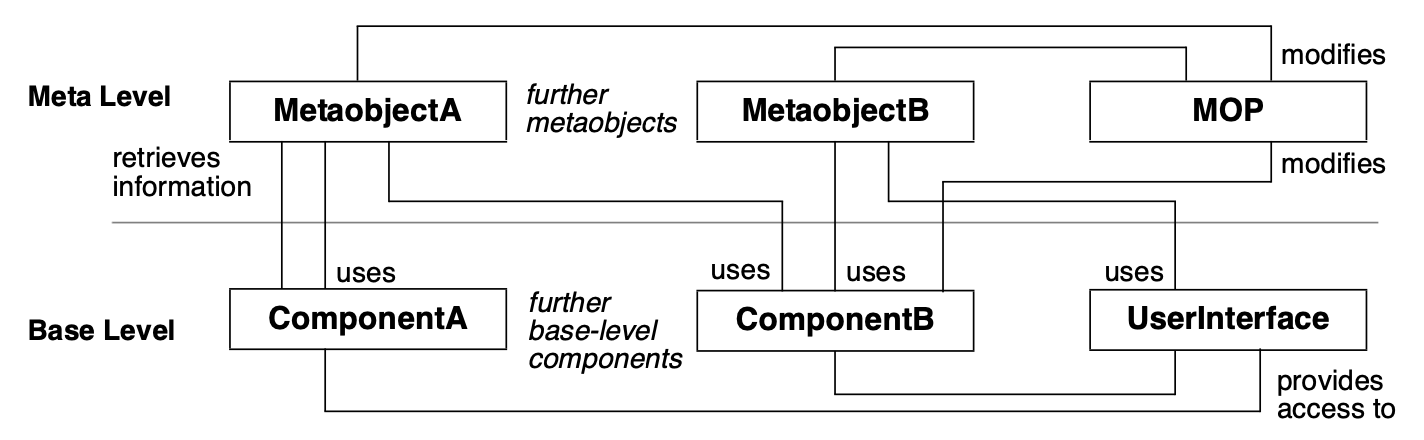
\includegraphics[width=1\textwidth]{Template_tesi/img/reflection.png}
    \caption{Architectural overview of a reflective system, illustrating the meta and base levels and their interactions. From \textit{Pattern-Oriented Software Architecture}, Buschmann et al.~\cite{Buschmann1996}.}
    \label{fig:reflection}
\end{figure}

In the context of this study, the presented pattern is fundamental as it allows for the dynamic management of a \textit{repository of meta-models}, without the need to define in advance the components with which the agents or the system will interact. As a result, agent interactions are dynamically modeled, leading to a structured cognitive workflow. In summary, a reflective approach yields the following key benefits:

\begin{itemize}[leftmargin=*, label=--] 

\item \textbf{Dynamic reconfiguration}: The system can adapt its behavior and structure at runtime based on changes to its meta-level, without requiring redeployment. 

\item \textbf{Separation of concerns}: By decoupling the application logic (Base Level) from the Knowledge Layer (Meta Level)—which is subject to more frequent changes—maintainability and extensibility are significantly improved.

\item \textbf{Semantic interoperability}: Components with no prior knowledge of each other can interact seamlessly. This enables the integration of heterogeneous agents into cohesive workflows, allowing the composition of complex and adaptive interactions.

\item \textbf{Explainability and traceability}: By observing the system’s components and behaviors, the meta-level establishes a foundation for a self-aware and auditable architecture. This allows the system to track its composition, explain the rationale for the decision, and trace the results.

\end{itemize}




\subsection{Integration of the Two-Fold Framework}


The novel and primary contribution of this work lies in integrating the Reflection Pattern, which provides structure and adaptability, with the AIBOM formalism, which ensures traceability. By coupling the comprehensive AIBOM inventory with the Reflection pattern, each cognitive workflow gains visibility into:

\begin{itemize}[leftmargin=*, label=--]
    \item \textbf{Its own structural elements} --- including agent composition, model versions, training data references, and external libraries.
    \item \textbf{Its meta-level} --- a supervisory layer that monitors changes, performs reconfiguration, and enforces security or compliance rules.
    \item \textbf{Runtime adaptations} --- triggered by environment changes, updates to agent dependencies, or new user requirements, all logged and documented within the AIBOM to maintain continuous traceability.
\end{itemize}

\noindent
This integration of reflection and AIBOM serves as the foundation for a self-aware and self-adapting multi-agent system. The architecture we propose includes:


\begin{itemize}[leftmargin=*, label=--]
    \item \textbf{Core AI Agents}: Responsible for distinct tasks (e.g., user intent detection, route planning, resource allocation).
    \item \textbf{Meta-Level Controller}: Dynamically adjusts agent configurations by referencing the AIBOM, ensuring only approved/compatible components are used.
    \item \textbf{AIBOM Repository}: Storing SBOM-like records for each AI component and its lifecycle events.
\end{itemize}

\noindent
By adopting this layered approach, we aim to demonstrate how cognitive workflows can be more traceable, transparent, and compliant with emerging AI regulations, especially where multi-agent collaboration requires detailed knowledge of each component’s provenance and behavioral characteristics.


\section{LLM-based System of Agents} 
\label{sec:AIBOM-system-of-agents}

AIBOM can be a valuable tool for managing complex systems composed of LLM agents by introducing the level of transparency and traceability typically associated with Software Bills of Materials. As foundation models rapidly transform the methodologies used to develop and deploy software-intensive systems, emerging approaches must embrace this shift by adopting novel architectural designs that address distributed, real-world scenarios rather than relying on conventional centralized solutions. In this context, the present study builds upon the work of Becattini, Verdecchia, and Vicario at the Software Technologies Laboratory, University of Florence \cite{becattini2025sallma}, extending their proposed \textbf{SALLMA} architecture.


\subsection{SALLMA Architecture Overview}
\label{sec:sallma}


\begin{figure}[h] 
    \centering
    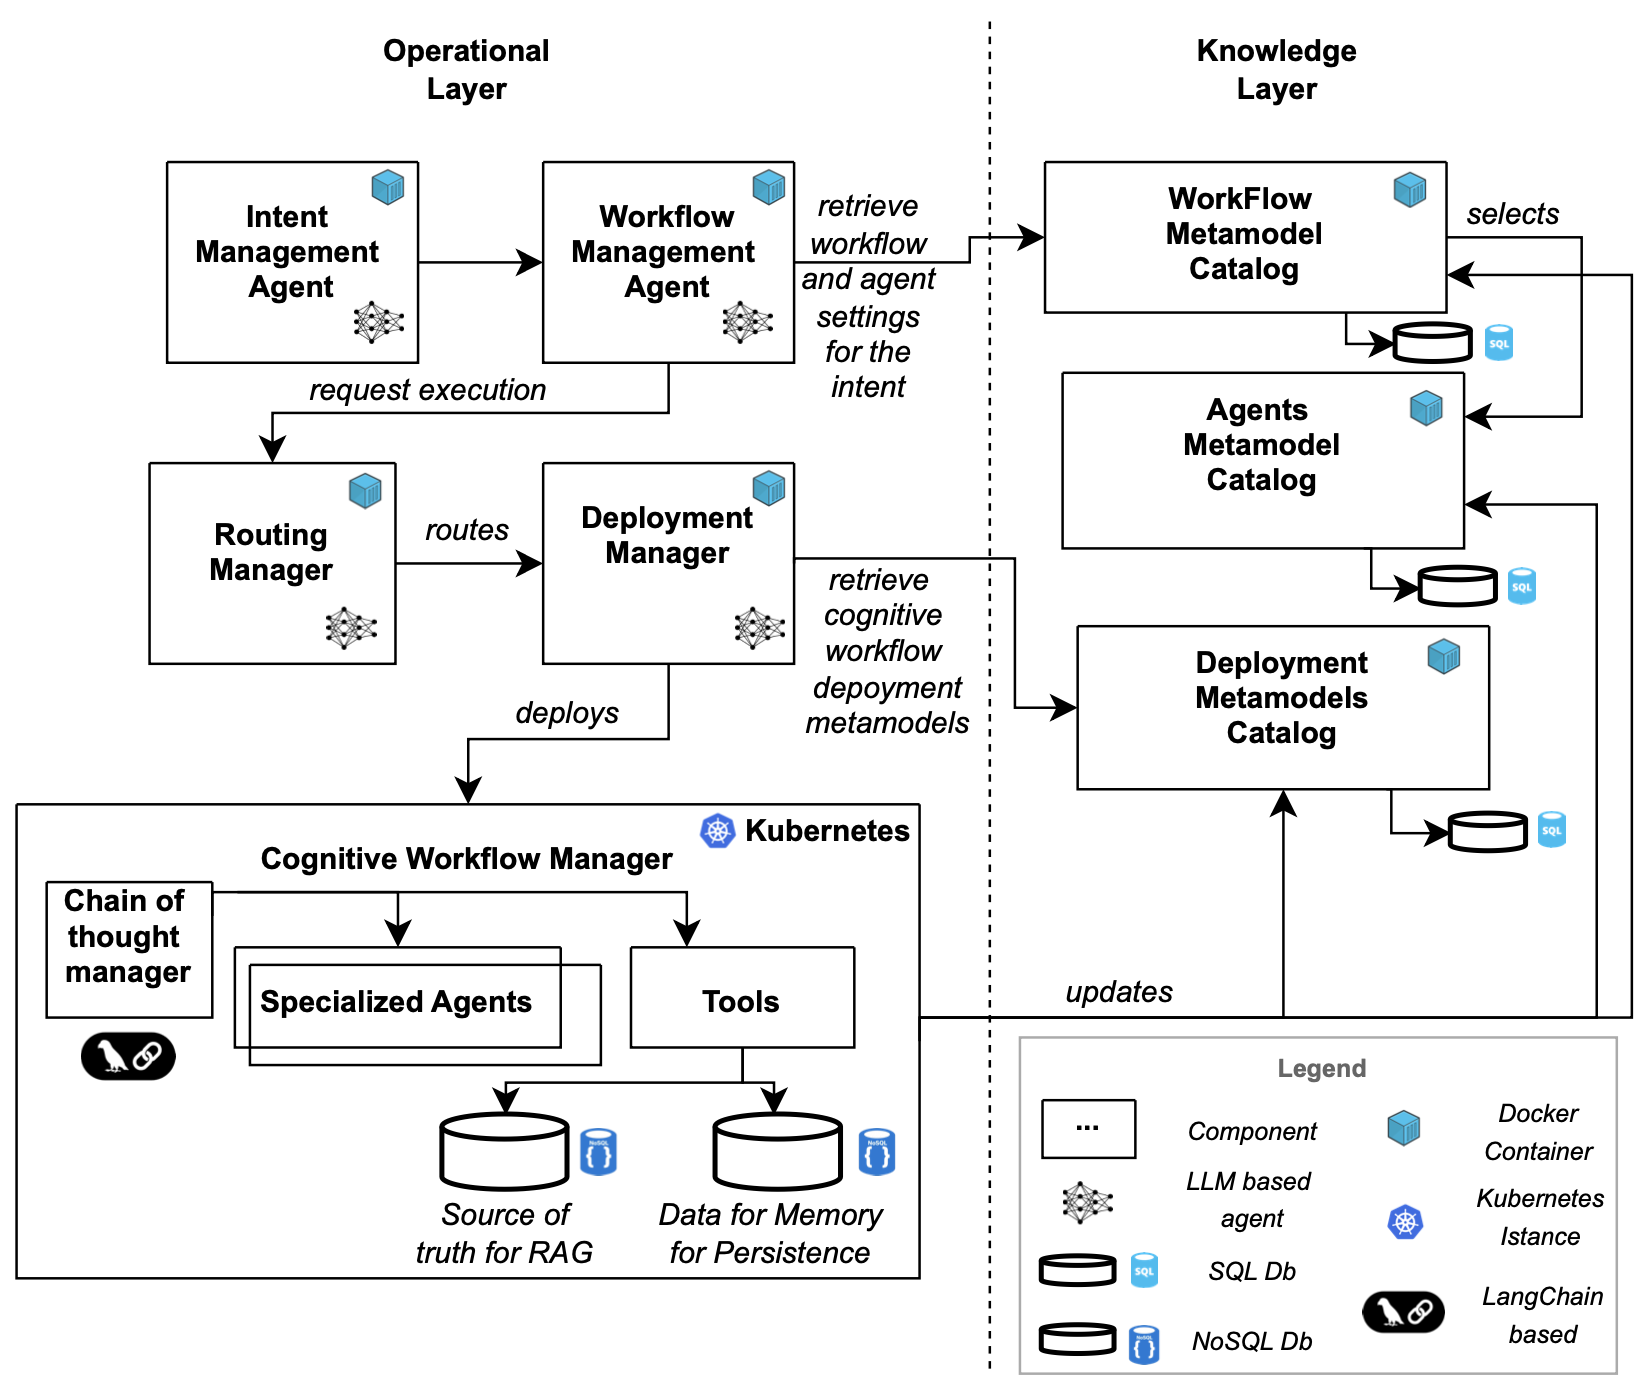
\includegraphics[width=.9\textwidth]{Template_tesi/img/SALLMA.png}
    \caption{SALLMA Architecture Overview}
    \label{fig:SALLMA}
\end{figure}
An introduction to the concept of SALLMA (Software Architecture for LLM-Based Multi-Agent Systems) will first be provided.
SALLMA  is a distributed, multi-agent architecture featuring an Operational Layer for real-time task execution and a Knowledge Layer for workflow and agent configuration meta-model management. Engineered from first principles, it is inherently modular and adaptive, designed to orchestrate multiple large language model (LLM) agents across both cloud and edge environments. While primarily a conceptual architecture, a proof of concept has been implemented to evaluate its functional suitability. 


By introducing a dual-layer structure, SALLMA addresses the limitations inherent in single-agent LLM systems, enabling dynamic adaptability of the system to the diversity of tasks in real-world applications. Notable limitations commonly observed in single-agent approaches include:

\begin{itemize}[leftmargin=*, label=--]
    \item Suboptimal hyperparameter configurations for specific requests.
    \item Lack of persistent memory.
    \item Limited access to ground-truth data.
    \item Challenges in reliability and sustainability management.
\end{itemize}

Compared to a single monolithic AI agent, an ensemble of specialized agents enables dynamic task decomposition and organic specialization: each agent can focus on its strengths, and tasks can be distributed dynamically across the system. Furthermore, this approach introduces fault tolerance: if one agent fails, others can continue execution, resulting in greater robustness and reliability.

A comprehensive overview of the SALLMA architecture is illustrated in Figure~\ref{fig:SALLMA}, highlighting the distinction between its two core layers. A brief explanation of each layer follows.

\subsubsection{SALLMA Operational Layer}

The Operational Layer acts as the dynamic core that is responsible for handling real-time interactions and orchestrating task-specific agents. Essentially, it is where the LLM agents “live” and interact, and is thus responsible for the decision-making process of the workflow. The primary elements of the Operational Layer are:

\begin{itemize}[leftmargin=*, label=--]
    \item\textbf{Intent Management Agent}: Parses the request and sets up the system to retrieve workflows using predefined intents stored in the Knowledge Layer.
    \item\textbf{Workflow Management Agent}: Breaks tasks into subtasks, assigning them to specialized agents.
    \item\textbf{Routing Manager}: Determines whether an existing workflow instance can handle the request or a new instance is required.
    \item\textbf{Deployment Manager}: Deploys workflows by leveraging the configurations and resources outlined in the Knowledge Layer.
    \item\textbf{Cognitive Workflow Manager}: Orchestrates tasks within a containerized environment, leveraging specialized agents, a chain-of-thought process, persistent memory for context-aware execution, and foundational data for reliable retrieval-augmented generation (RAG).
\end{itemize}





\subsubsection{SALLMA Knowledge Layer}
The Knowledge Layer is dedicated to storing and managing information that agents use or produce. It serves as the foundation for SALLMA's meta-model management, maintaining an inventory of reusable workflows and agent configurations. Agents in the Operational Layer rely on the Knowledge Layer both to retrieve relevant data and to update it with new findings or changes in state. Among its components, the most notable include:

\begin{itemize}[leftmargin=*, label=--]
    \item\textbf{Workflow Metamodel Catalog}: Stores predefined workflow configurations optimized for different tasks.
    
    \item\textbf{LLM Configuration Catalog}:  Contains predefined configurations for each LLM agent (e.g., hyperparameters, resource allocations, and so on).

    \item\textbf{Deployment Metamodels Catalog}: Holds a set of deployment models that detail the proper cognitive workflow configurations for each operational scenario (e.g., cloud or edge environments).
\end{itemize}






\subsection{Extending SALLMA}
\label{sec:ext-sallma}


The proposed framework integrates SBOM management into the SALLMA multi-agent system architecture. By extending SALLMA, we introduce a systematic way to document and track the composition of each agent within the Knowledge Layer and to use that data in the Operations Layer for better decision-making and security inspections. In contrast to traditional practices that rely on the static generation of SBOMs and their passive use for tracking dependencies, this novel approach marks a paradigm shift toward dynamically leveraging SBOM knowledge within the system across its entire lifecycle. The key idea is that as the multi-agent system evolves, it will generate and maintain an SBOM that describes all its software components (agents, models, libraries, and dependencies); this self-describing inventory of components information will be actively used by the system for governance and maintenance, enhancing trust in what the AI is executing.

A limitation of the approach outlined in SALLMA is the lack of a clear formalization regarding information ownership, specifically whether it should reside within the Knowledge Layer or be delegated to external systems and accessed via retrieval augmented generation (RAG).
In this context, an AIBOM approach could be beneficial, as it allows a more proper and elegant differentiation between the knowledge layer—where meta-models of the cognitive workflows are stored—and the data level, where data belongs.






\section{System's Design and Implementation}\label{sec:design-and-implementation}

The following section details the architecture and core components of the proposed system in its design and final implementation. Building on the conceptual foundations introduced earlier, it outlines the structural patterns, persistence strategies, execution mechanisms, and dynamic adaptation features that enable the orchestration of cognitive workflows. Every design choice is motivated by the need for extensibility, modularity, and runtime flexibility in managing AI agents and their meta-structures. The demonstration implementation is carried out in Java, leveraging the emerging Spring AI framework from the Spring ecosystem to support AI engineering tasks (see Appendix \ref{ch:appendix_spring} for a detailed explanation of this choice). As a proof of concept, although SALLMA was conceived as a distributed architecture, the concrete implementation proposed to support the study is based on a single application where workflow nodes are instantiated in memory rather than deployed as separate services. This simplification maintains the core concepts while allowing for comprehensive validation of the system's logic and interaction patterns.






\subsection{Pattern Outline}


As previously introduced, the proposed architecture adheres to the SALLMA philosophy, adopting a dual-layered structure comprising the Knowledge Layer and the Operational Layer. Leveraging the Reflection Pattern alongside aggregation and subclassing, the architecture achieves a high degree of flexibility.
The Operational Layer hosts the execution-time entities: instance nodes and workflows; each instance is linked to a corresponding meta-model, which belongs to the Knowledge Layer and governs its actual runtime behavior. Across both layers, as illustrated in Figure \ref{fig:nodes-reflection-uml}, specialized nodes encapsulate different AI models and external tools (e.g., LLMs, Embedding Models, RESTful Services, Vector Databases, etc.).

\begin{figure}[h]
    \centering
    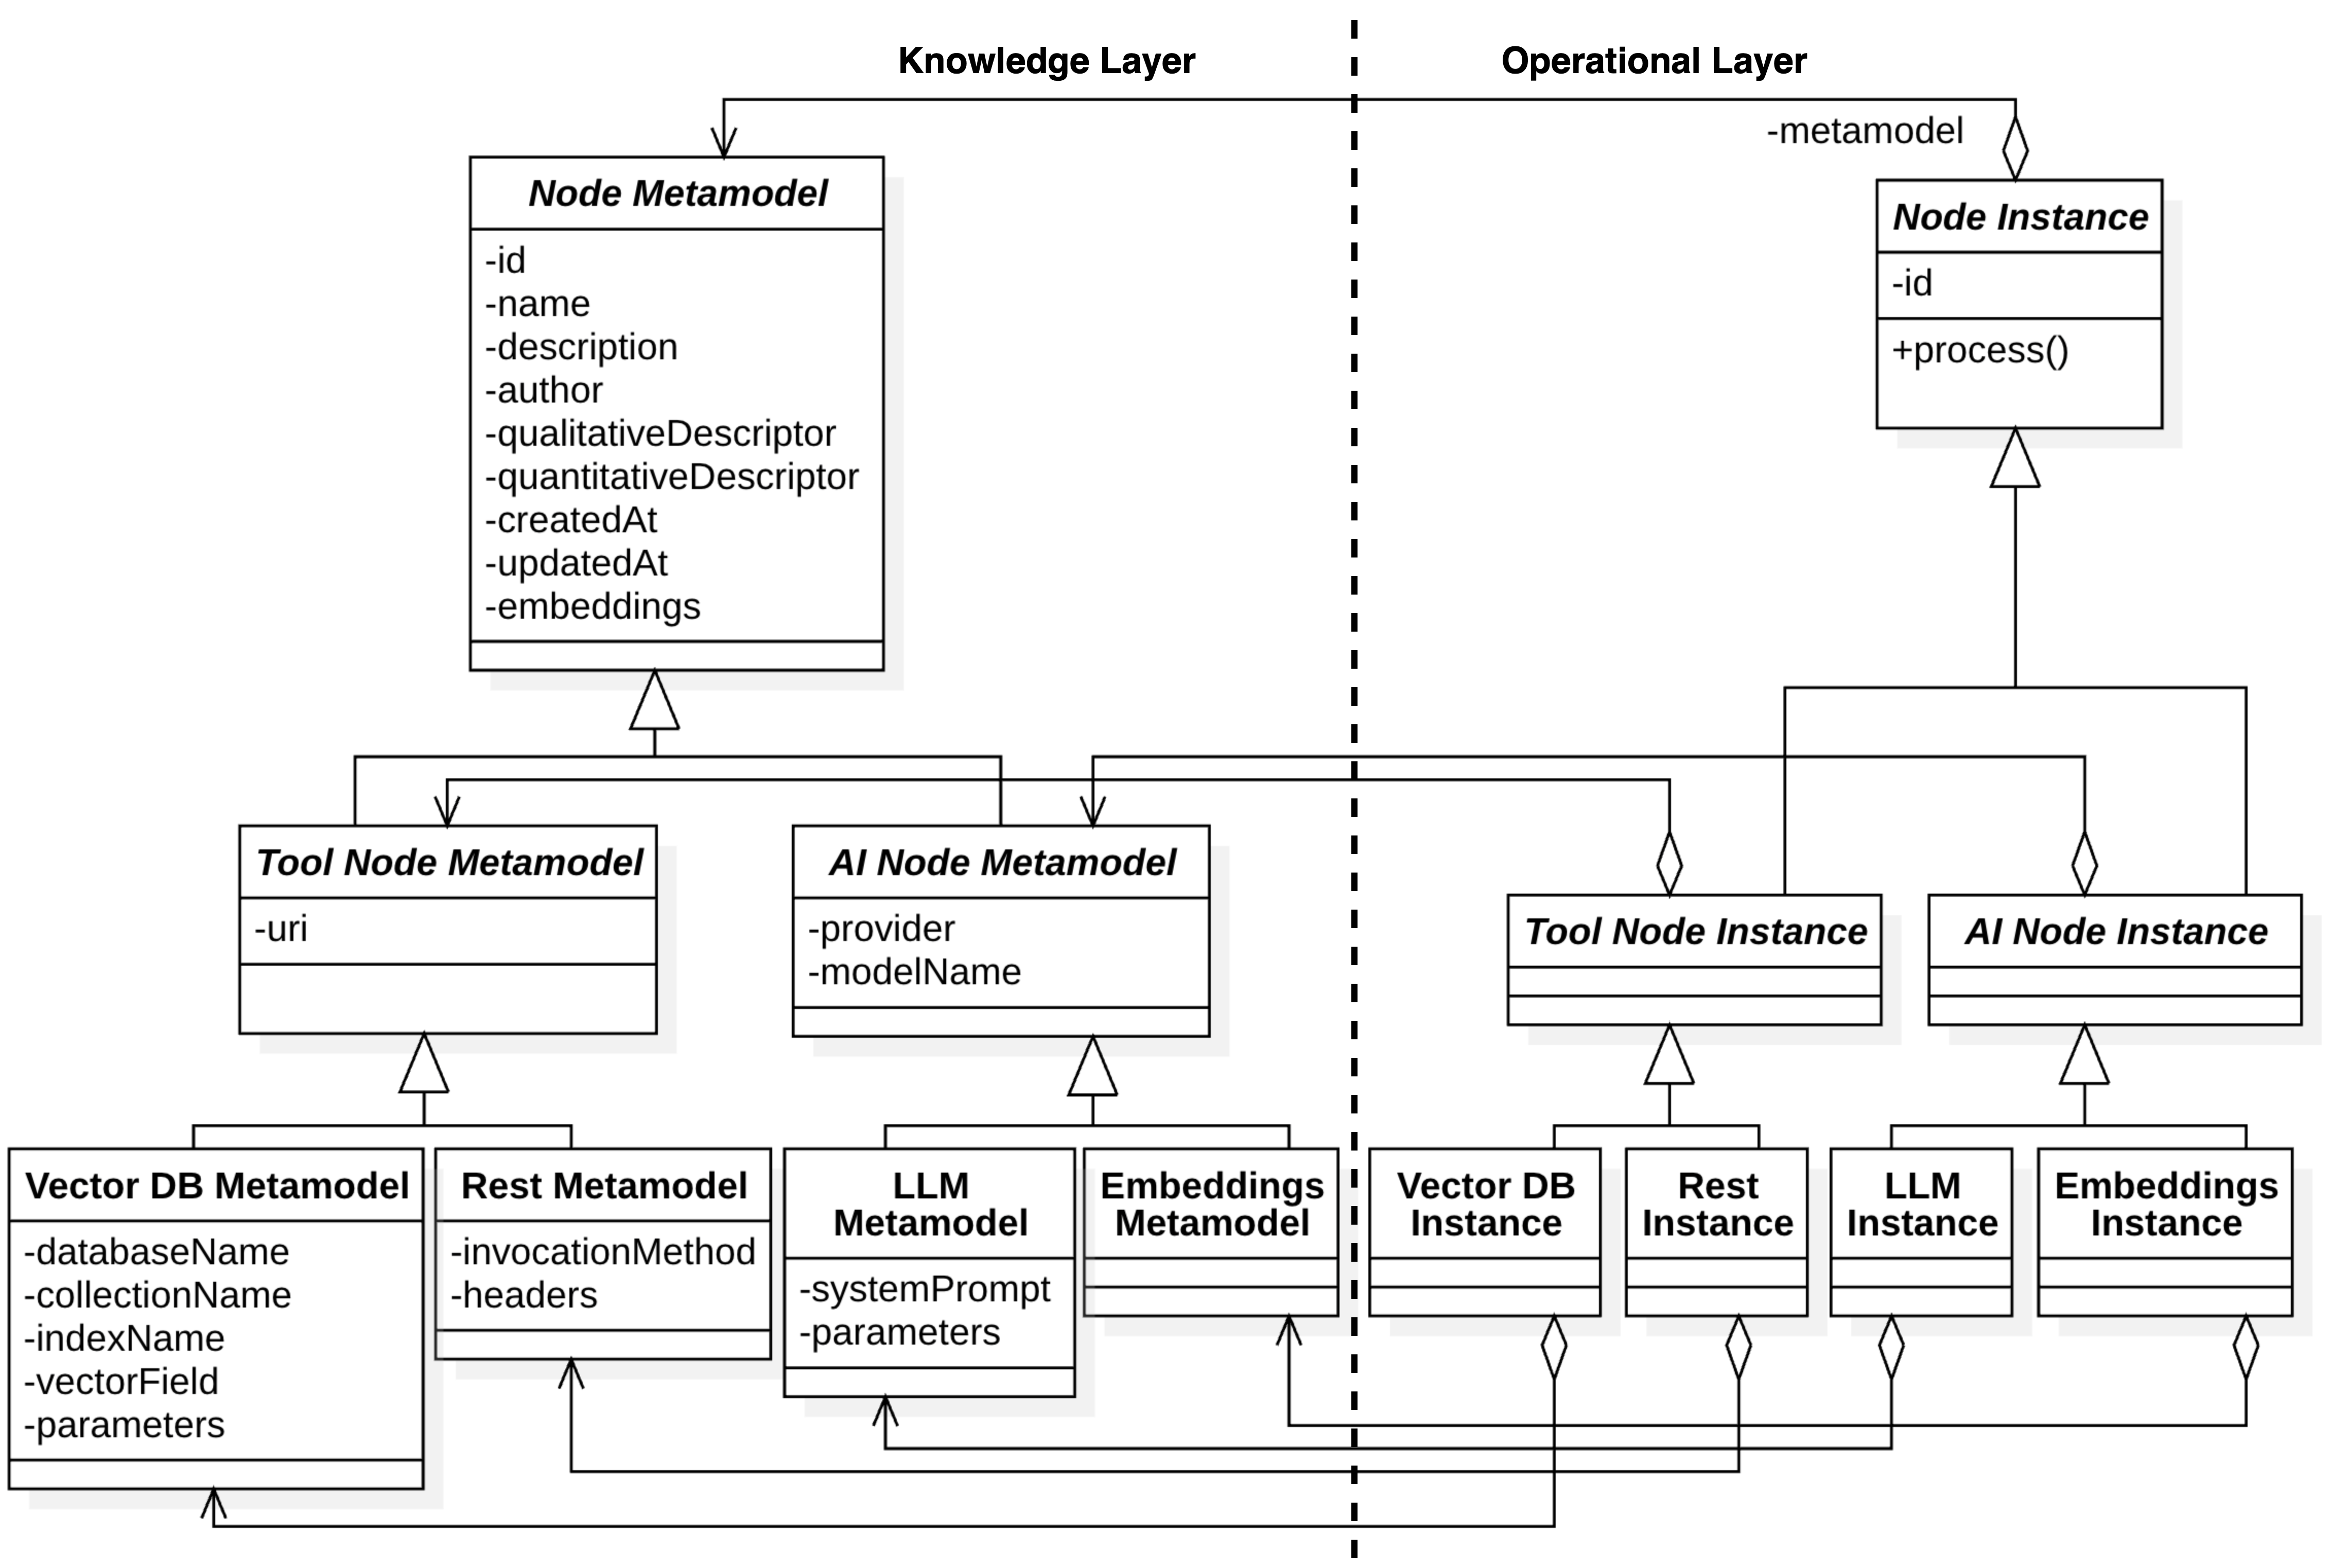
\includegraphics[width=1\textwidth]{Template_tesi/img/nodes-reflection-uml.png}
    \caption{Dual-layer architecture diagram showing Knowledge Layer meta-models (left) and their corresponding Operational Layer instances (right), illustrating the inheritance relationships between components.}
    \label{fig:nodes-reflection-uml}
\end{figure}


The nodes can be combined into workflows, which are essentially \textit{directed acyclic graphs} (DAGs). Each workflow is represented as a graph consisting of nodes and edges, where nodes correspond to specific meta-models with their associated versions, and edges define the connections between nodes within the workflow structure.
Ideally, multiple workflows can be composed together, allowing simple workflows to be reused and integrated into more complex processing pipelines. For example, the Retrieval-Augmented Generation\footnote{RAG is an AI engineering technique used to retrieve information from an external knowledge base in order to ground LLMs on accurate and up-to-date data.} (RAG) pattern can be modeled as a sub-workflow consisting of the following nodes:

\begin{enumerate}[leftmargin=*, label=\textbf{\arabic*.}]
    \item \textbf{Embedding node}: Calls an embedding model to generate a vector representation of the text input.
    \item \textbf{Vector database node}: Performs a vector similarity search against a pre-indexed data repository.
    \item \textbf{LLM node}: Receives the original query along with the retrieved documents and generates a final response.
\end{enumerate}


\begin{figure}[h]
    \centering
    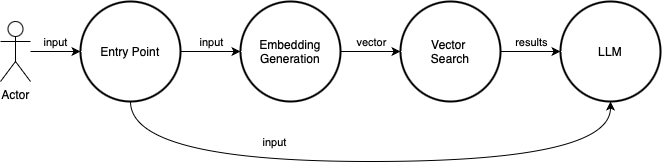
\includegraphics[width=.9\textwidth]{Template_tesi/img/RAG-workflow.png}
    \caption{Diagram of the RAG pattern workflow corresponding to the embedding, retrieval, and generation steps.}
    \label{fig:RAG-workflow}
\end{figure}










\subsubsection{Data Persistence}

A MongoDB database was selected for the meta-models repository due to its NoSQL, document-based approach. This choice is ideal for schema flexibility, especially when dealing with the evolving and heterogeneous data common in multi-agent configurations (e.g., varying parameters, node types, and data formats). Its nested structure also provides efficient storage for SBOMs. Finally, the out-of-the-box Vector Search capability provided by Atlas\footnote{\url{https://www.mongodb.com/atlas} - a fully managed Database-as-a-Service (DBaaS) provided by MongoDB.} was key in enabling semantic search for RAG, without requiring additional dedicated databases. The system uses three collections to manage:

\begin{itemize}[leftmargin=*, label=--] 
    \item The meta-models of individual nodes
    \item The meta-modes of workflows
    \item The catalog of intents handled by the system
\end{itemize}

\noindent

Although inheritance in entity modeling can add complexity to data persistence, the combination of \texttt{Jackson}’s polymorphic deserialization and \texttt{Spring Data MongoDB} effectively abstracts away this complexity. When a subclass instance is persisted, Spring automatically includes a \texttt{\_class} field in the document, which contains the fully qualified class name. This allows the framework to correctly deserialize the document and resolve the appropriate subclass during    \textit{Object-Document Mapping} (ODM).




\subsection{Structured Data Flow}


In workflow-based systems, controlling the flow of data between components is essential to ensure consistency and interoperability throughout the execution. In the context of this work, we utilize the notion of ports as an abstraction to declare the input and output interfaces of each node within the workflow. This construct promotes modular design, enables validation during data propagation, and assists in the early detection of incompatibilities. To enforce the structural correctness of meta-models, dedicated services are employed to verify the compatibility of ports across connected nodes, ensure type consistency, and validate the satisfaction of all required inputs.

\subsubsection{Input and Output Ports}

Ports act as standardized entry and exit points for data within a node.
A port is identified by a unique key and is defined by a schema that describes the expected data type and structure (e.g., primitive types, objects, arrays), supporting rich and flexible data modeling. Additionally, the port abstraction supports various specialization types which encode domain-specific semantics. For instance, in nodes representing RESTful services, ports can correspond to request body fields, query parameters, path variables, etc. In contrast, LLM-based nodes might define ports in terms of system prompt variables or user messages. An overview of the class structure used to define ports and their schema is provided in Figure~\ref{fig:port}. 


\begin{figure}[h]
    \centering
    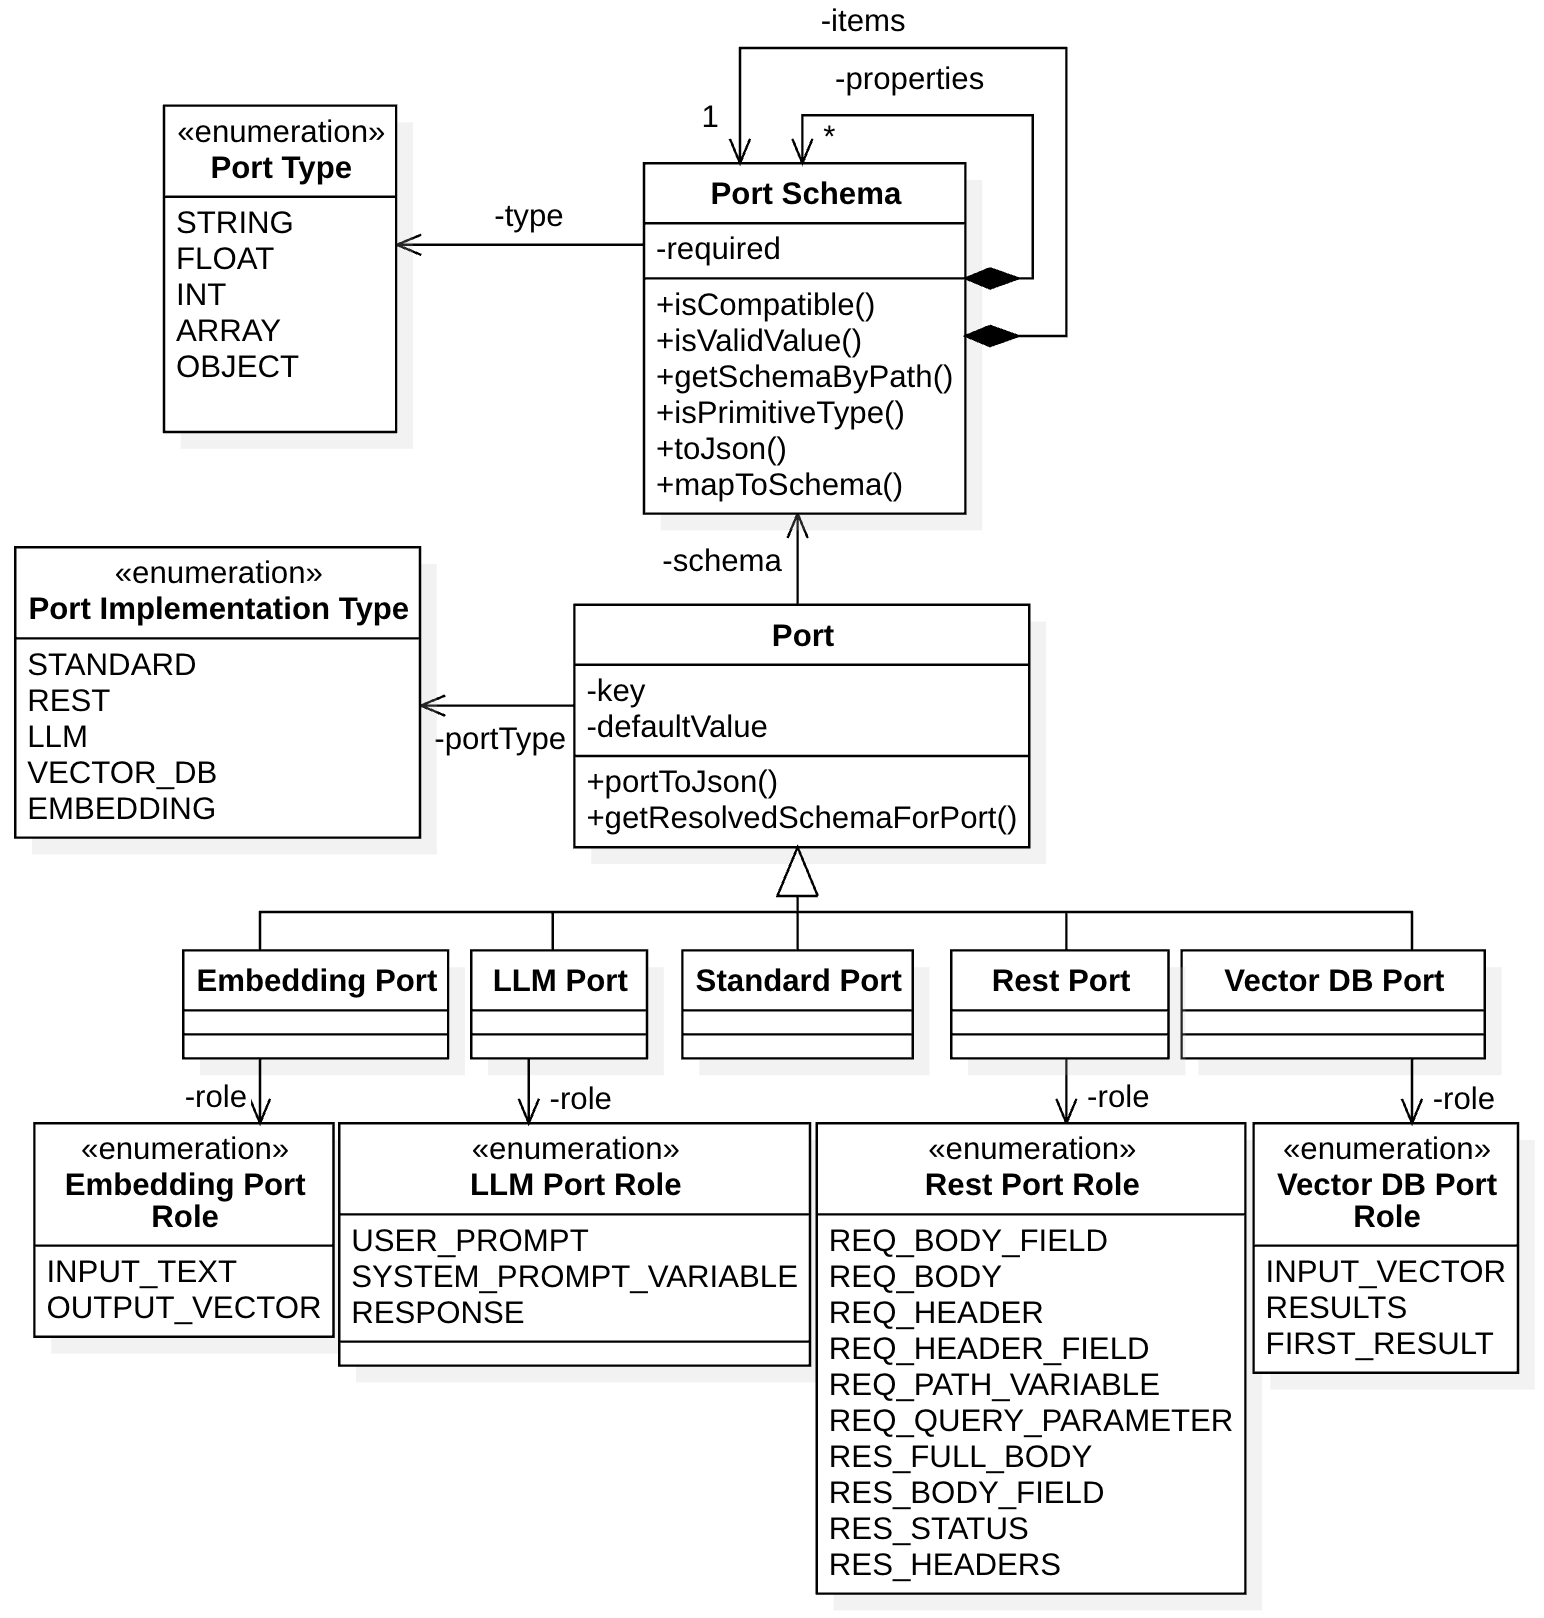
\includegraphics[width=0.8\textwidth]{Template_tesi/img/port-uml.png} 
    \caption{UML Class Diagram illustrating the \textit{Port} and \textit{Port Schema} entities, which define the structure and behavior of inputs and outputs for workflows' nodes. For brevity, the figure omits that each port implementation is associated with a corresponding builder class.
}
    \label{fig:port} 
\end{figure}



\subsubsection{LLM Structured Outputs}

When working with Large Language Models (LLMs), generating structured outputs is critical to ensure predictable consumption of the model’s responses. Spring AI addresses this need through its \textbf{Structured Output API} \cite{tzolov2024structured}, which includes a set of \textbf{Structured Output Converters}. These converters transform raw models' output into instances of predefined Java classes, leveraging prompt engineering\footnote{The process of designing inputs to effectively guide generative AI models toward desired outputs.} to guide the model's formatting behavior. Essentially, as shown in Figure~\ref{fig:structured-output-spring}, instructions are embedded in the prompts to shape the output according to the expected structure, following which the converter parses the response into a Java object.
Nevertheless, as meta-model's ports are dynamically typed and their schema is more expressive than what Spring AI supports natively, a custom converter layer was developed. This layer, built on top of the one of Spring AI,  also leverages prompt augmentation\footnote{A prompt engineering technique that enriches a base input prompt by adding context, examples, or instructions to improve the relevance, accuracy, or specificity of the AI's response.} to map the LLM responses to the corresponding output port schema declared in the meta-model.

\begin{figure}[H]
    \centering
    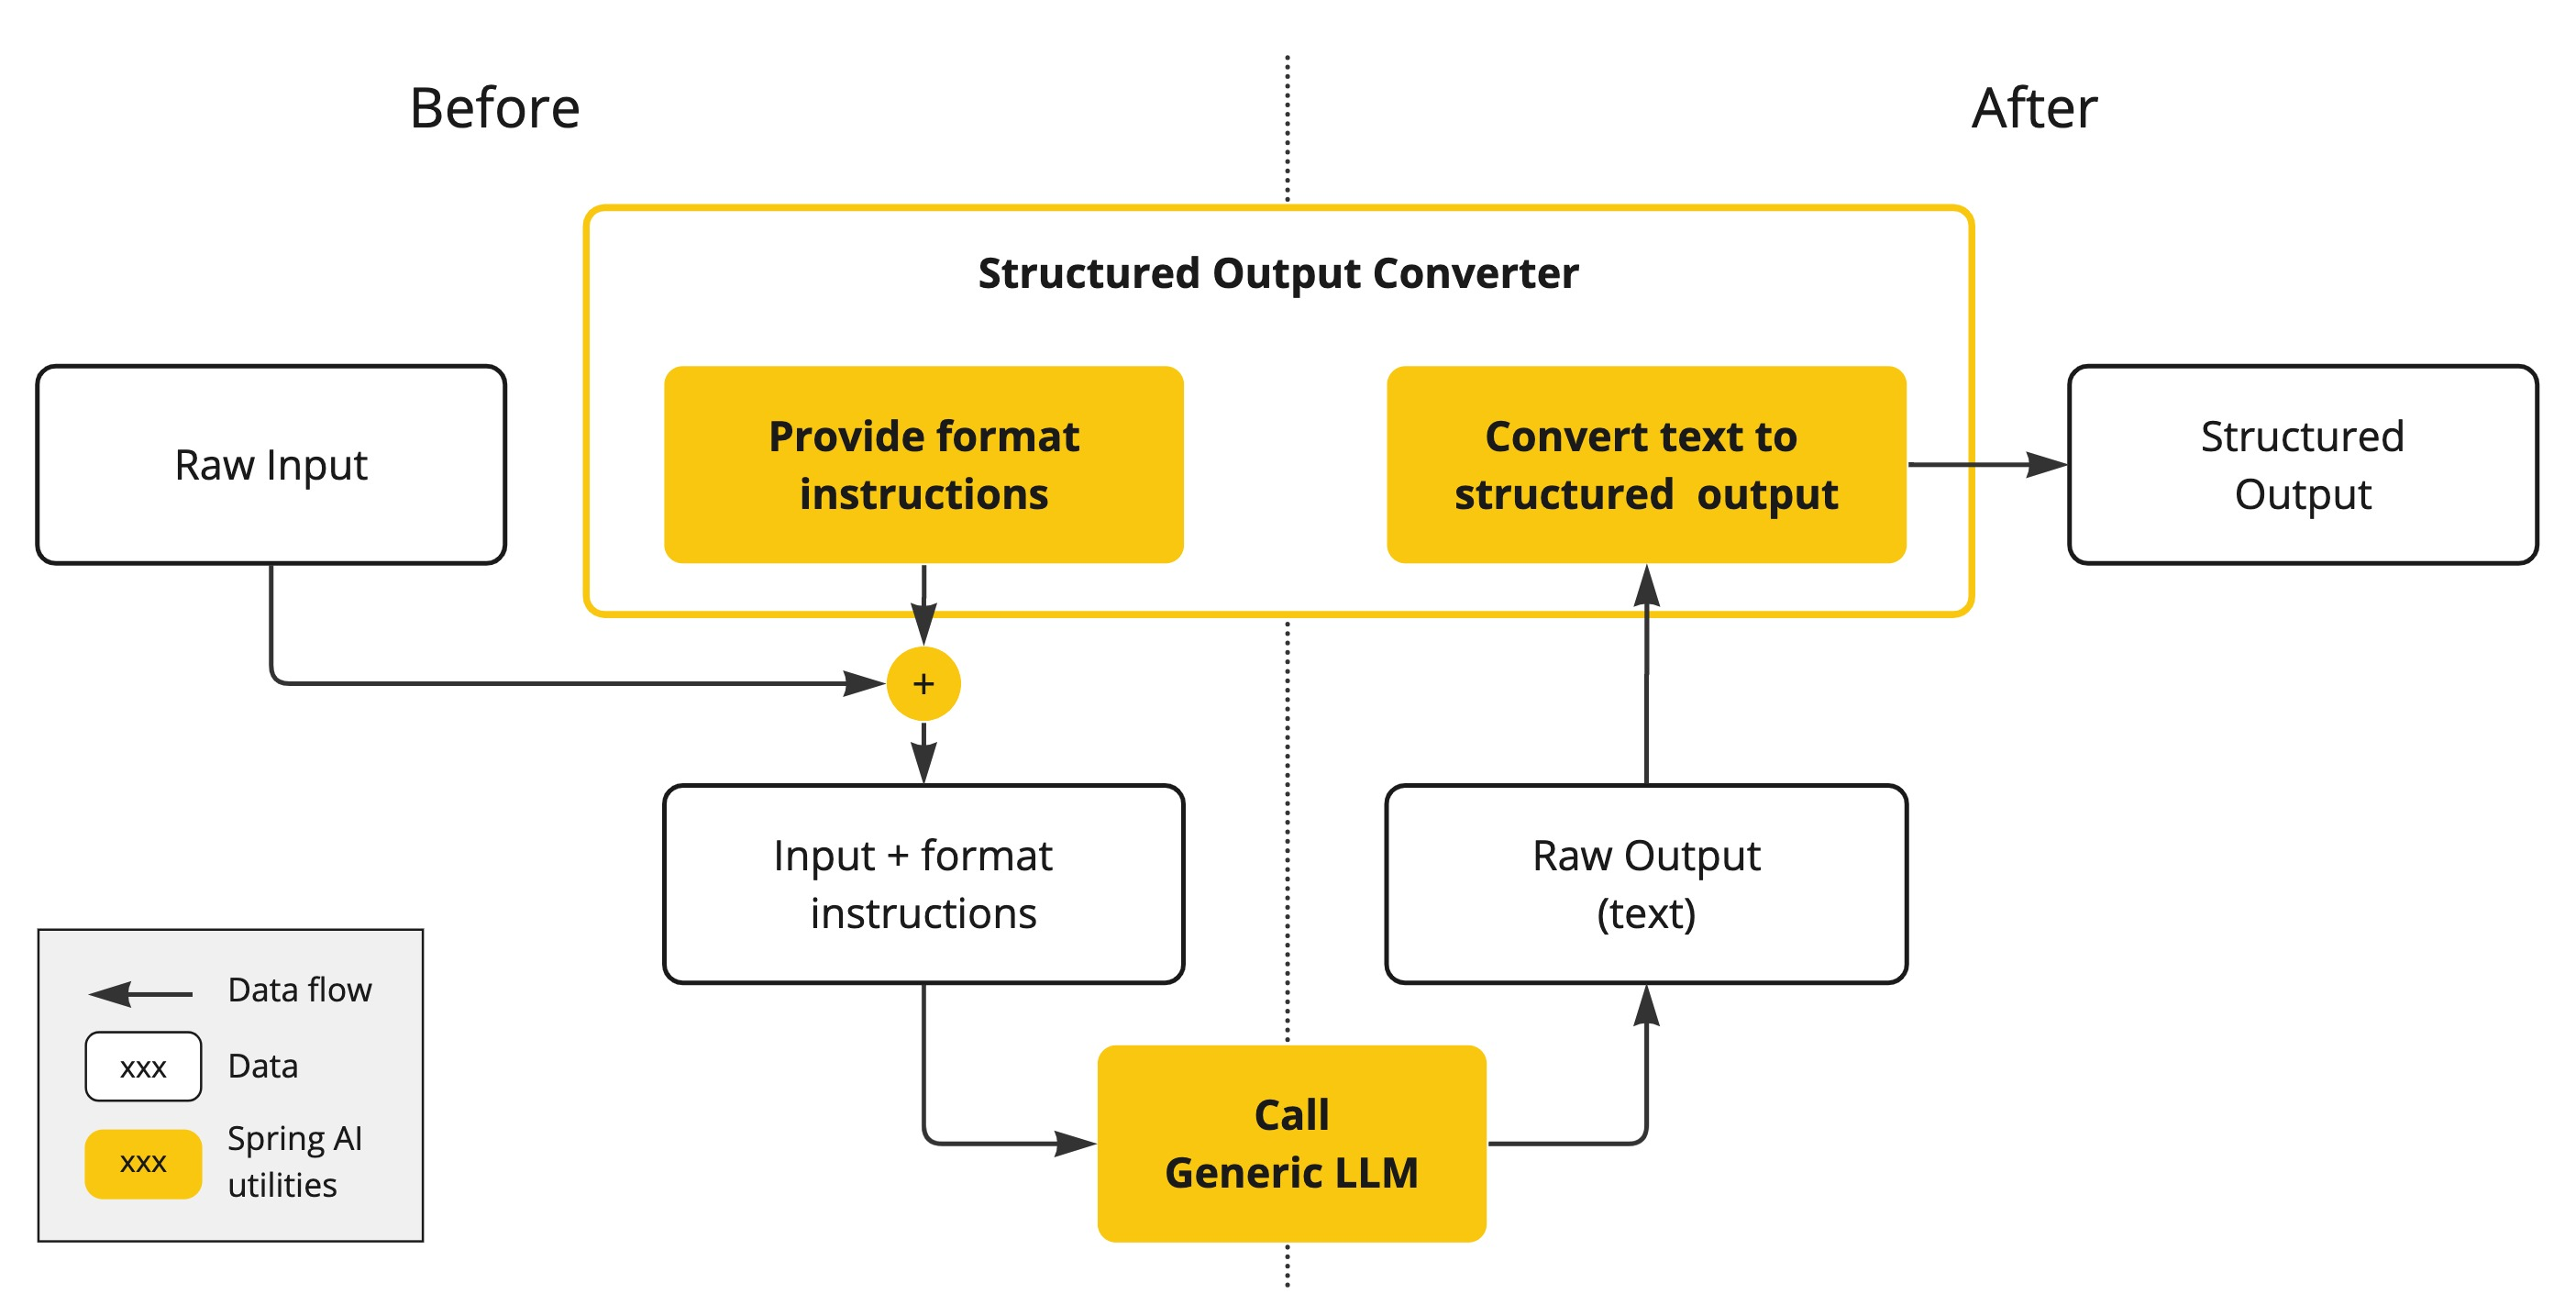
\includegraphics[width=1\textwidth]{Template_tesi/img/structured-output.jpg}
    \caption{Overview of Spring AI's Structured Output Converters. From \url{https://spring.io/blog/2024/05/09/spring-ai-structured-output}}
    \label{fig:structured-output-spring} 
\end{figure}




\subsubsection{Edge Bindings} \label{sec:bindings}
A central concept to facilitate the collaboration of nodes within workflows is the idea of bindings. These specify how the output of one node connects to the input of the following node. This is particularly important in heterogeneous systems where different nodes might use different naming conventions or data formats for interface ports. Bindings operate in two modes:

\begin{itemize}[leftmargin=*, label=--]
    \item \textbf{Explicit Bindings}: These are direct mappings between input and output port names. As aliases, they allow ports with different names to be connected explicitly.
    \item \textbf{Implicit Matching}: When no bindings are provided, the system attempts to connect ports with the same key name, assuming their schema is compatible. 
\end{itemize}


This mechanism is essential for enabling interoperability between components provided by different vendors or when combining general-purpose nodes with more specialized ones. Importantly, while bindings can be manually defined at design time, they can also be determined dynamically at runtime through the use of an LLM-based agent. In our implementation, this agent is referred to as the \texttt{Port Adapter Service}, which enables the adaptiveness of the system. The service takes as input the schemas of two port sets—source and target—and generates a bindings map by matching fields based on names, types, structure, and required fields. It supports nested objects through dot notation\footnote{Dot notation is a syntax used to access nested fields in structured data (e.g., \texttt{user.address.city}), commonly found in formats like JSON or object schemas.} and applies renaming where needed to ensure schema alignment.




\subsection{Workflow Execution} \label{sec:execution}

For the purposes of this project, the workflow engine was built entirely from the ground up, despite considering alternatives like \textit{n8n}\footnote{
n8n is a workflow automation tool. See \url{https://n8n.io/}}.
While the Operational Layer is the core of the system—where the actual execution of workflows takes place—it heavily relies on the Knowledge Layer. As shown in Figure \ref{fig:exec}, the Knowledge Layer is accessed through the \textit{MOP} (Meta Object Protocol), as already introduced in Section \ref{sec:reflection}. The MOP encapsulates meta-model services that directly interface with the three repositories: Metamodel Catalogs of Workflow, Nodes, and Intents. Therefore, the MOP acts as the controller of meta-models and provides the only possible way for the Operational Layer to fetch and update them. Additionally, it handles event dispatching and, through dedicated services such as the \texttt{Workflow Metamodel Validator} and \texttt{Node Metamodel Validator}, ensures the structural integrity of these meta-objects. The complete execution process proceeds as follows:

\begin{enumerate}[leftmargin=*, label=\textbf{\arabic*.}]
    \item\textbf{Intent Detection}: \texttt{The Intent Detection Service} identifies the user's intent from natural language input. It retrieves relevant intents from the Knowledge Layer for RAG and extracts unstructured variables. If no matching intent exists, it creates a new one with associated metadata.
    \item\textbf{Workflow Selection}:  The \texttt{Routing Manager} selects a workflow corresponding to the detected intent by querying available workflows. If multiple matches are found, selection can be guided by intent-specific scores—derived from user feedback, comparative evaluation, or an \textit{AI judge}\footnote{An AI model that is used to evaluate the output of other AI systems \cite{huyen2024ai}}—while a temperature-based sampler ensures diversity in the final choice.
    \item\textbf{Workflow Retrieval}: The \texttt{Workflow Instance Manager} retrieves an existing workflow from the registry or instantiates a new one if none exists by fetching up-to-date information from the Knowledge Layer.
    \item\textbf{Workflow Execution}: The \texttt{Input Mapper Service} (LLM-powered) binds the extracted input data to the entry ports of the workflow. The \texttt{Workflow Executor} then runs the process, supported by the \texttt{Port Adapter Service} (LLM-powered), which resolves any port mismatches experienced during execution.
\end{enumerate}


\begin{figure}
  \centering
  \begin{adjustbox}{center}
    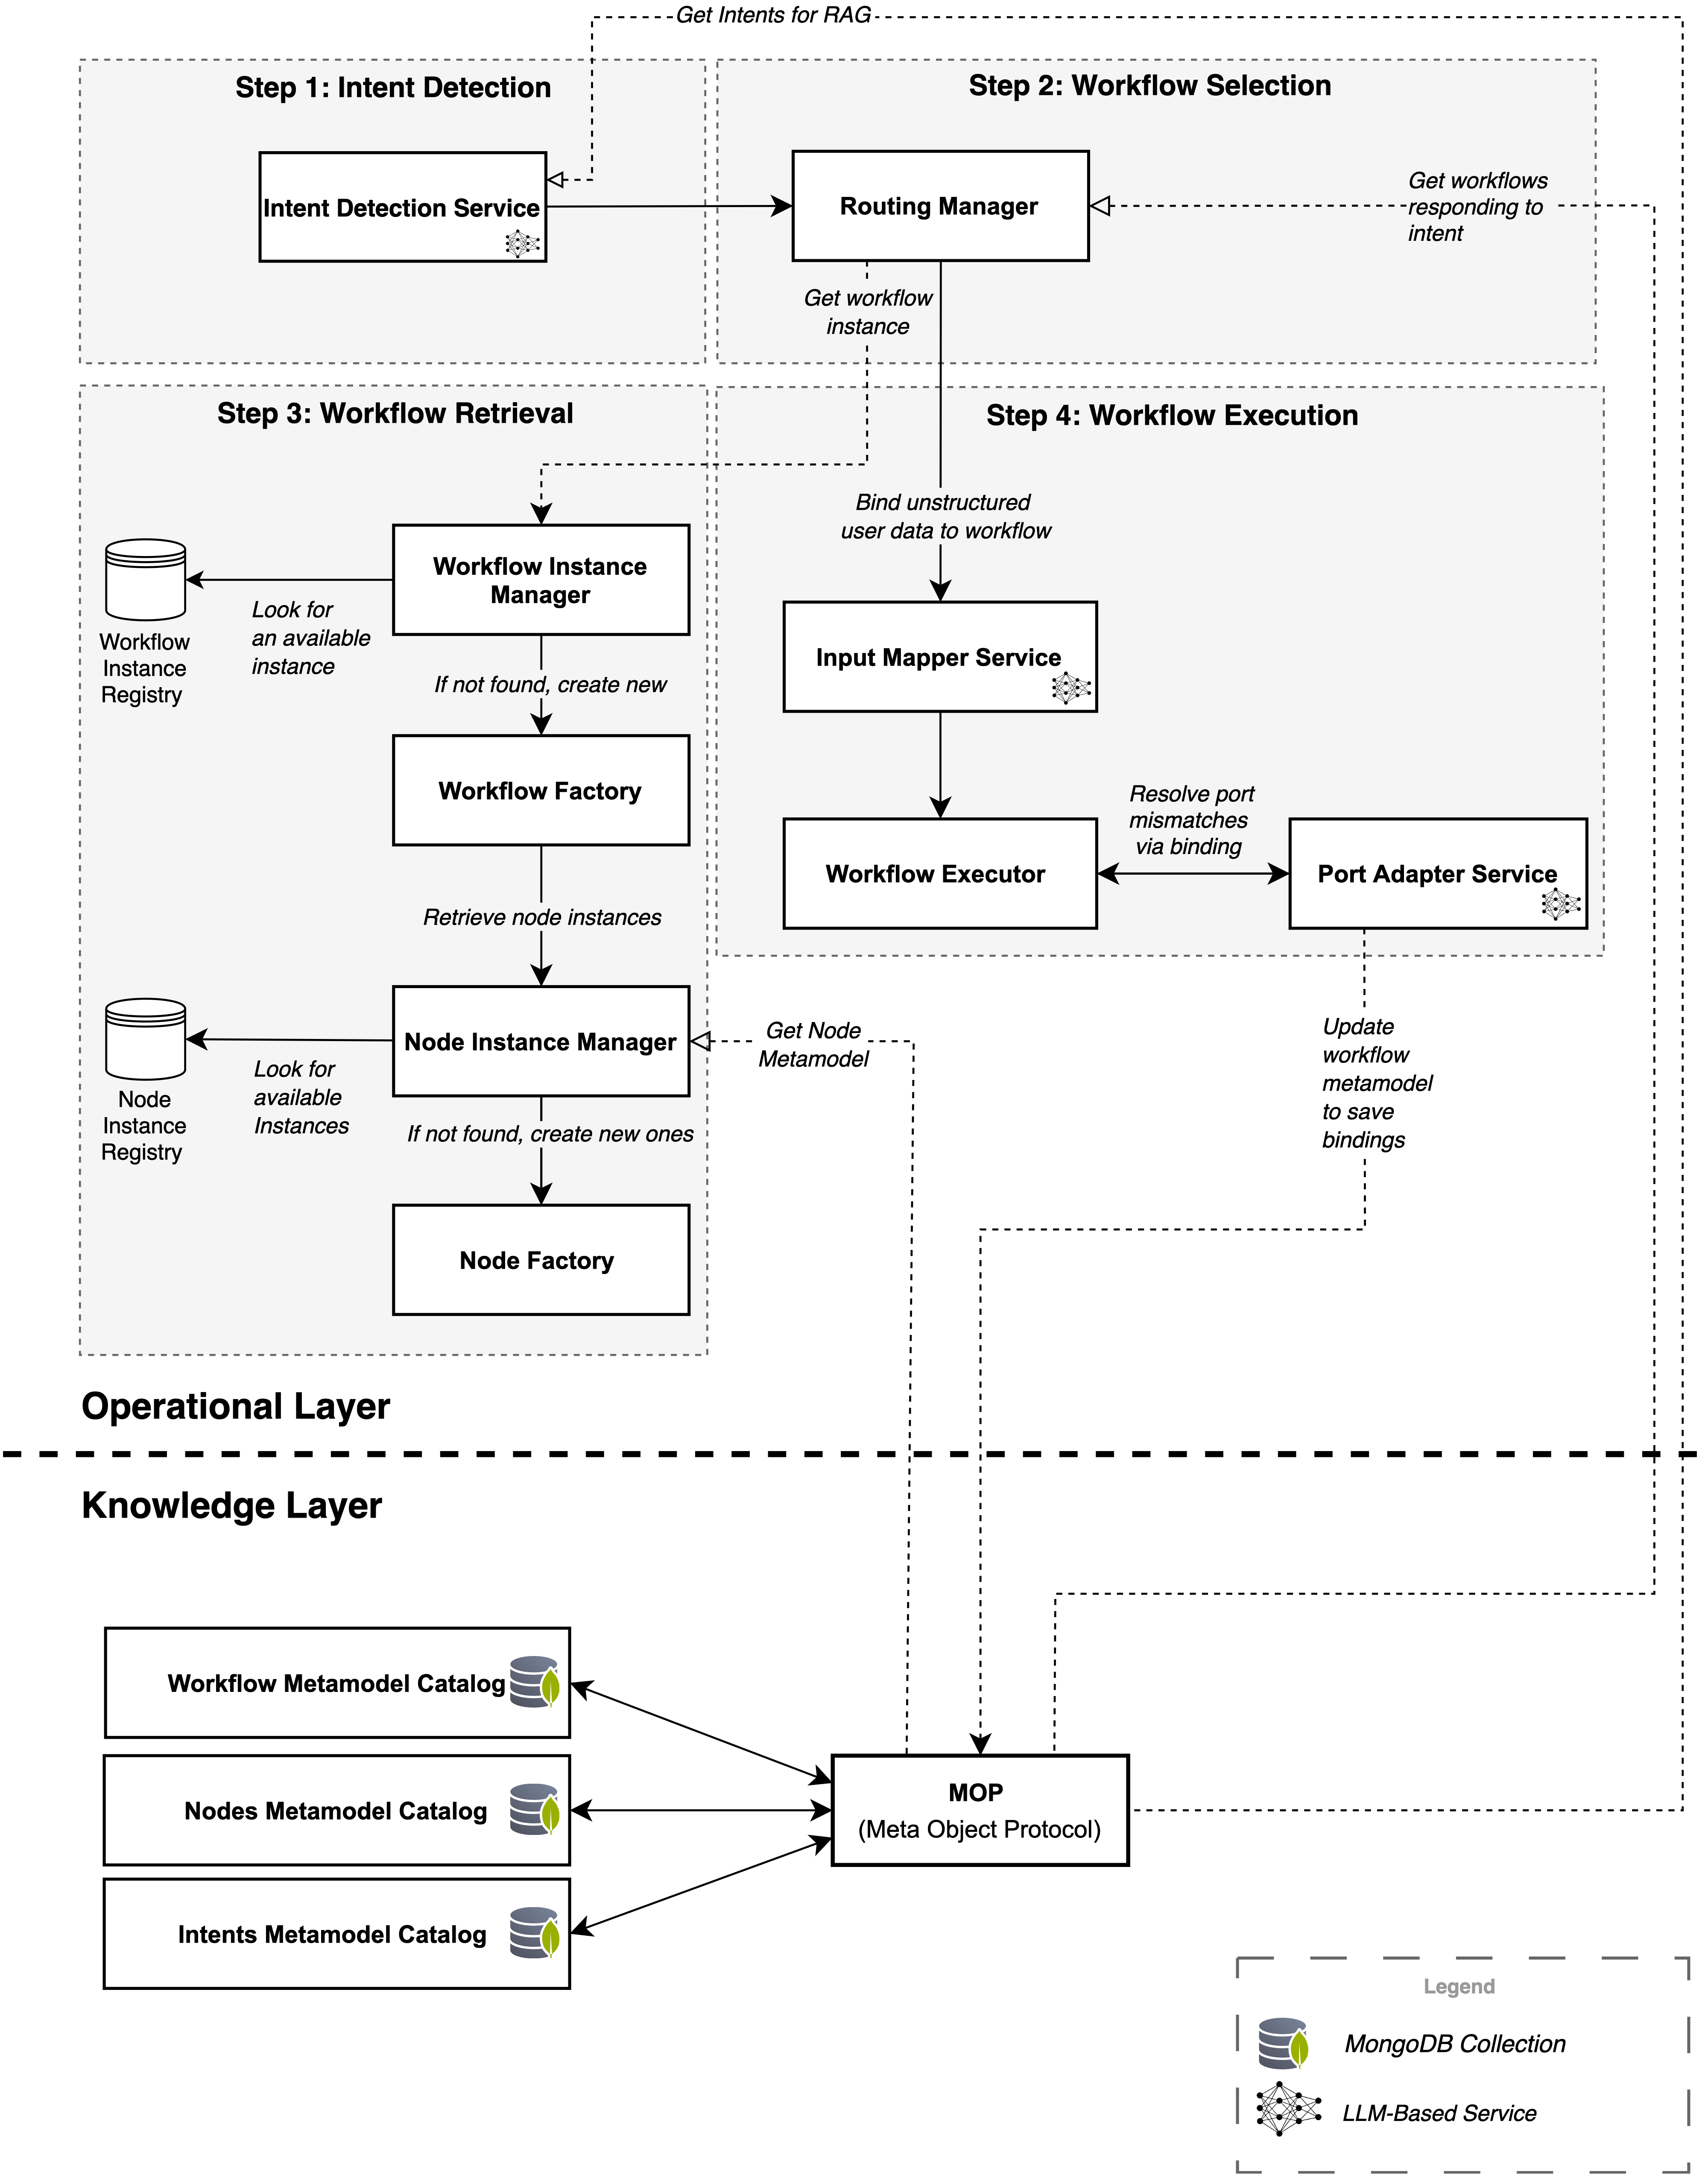
\includegraphics[width=1.2\textwidth]{Template_tesi/img/execution.png}
  \end{adjustbox}
  \caption{Workflow Execution four-step process, showing the interaction between the Operational Layer components and the Knowledge Layer accessed through the MOP and its three meta-model catalogs.}
  \label{fig:exec}
\end{figure}


\subsubsection{Ports Adaption}

As previously mentioned, the \texttt{Port Adapter Service} is essential for ensuring system adaptability and the interoperability of components, even when these components are developed independently or by third-party vendors. Since nodes are not necessarily aware of each other, aligning components with mismatched input and output interfaces is critical to achieving component reusability.
As discussed in Section \ref{sec:bindings}, edge bindings between components can be resolved at runtime. This task is handled by the \texttt{Port Adapter Service}, which is triggered by the \texttt{Workflow Executor} whenever a node about to be executed lacks the necessary input data in the current execution context. If a functional adaptation is found, the Operational Layer interacts with the Knowledge Layer to update the workflow meta-model. As a result, following executions of the same workflow will skip the adaptation step, reducing execution time. Figure \ref{fig:adaption-flow-chart} provides a summary of this dynamic adaptation process.
Ultimately, this mechanism significantly improves the \textbf{resilience of the system}: when a workflow depends on a node whose interface changes (e.g., due to a breaking change), the system can attempt to automatically resolve any incompatibilities introduced by that change.

\begin{figure}[h]
    \centering
    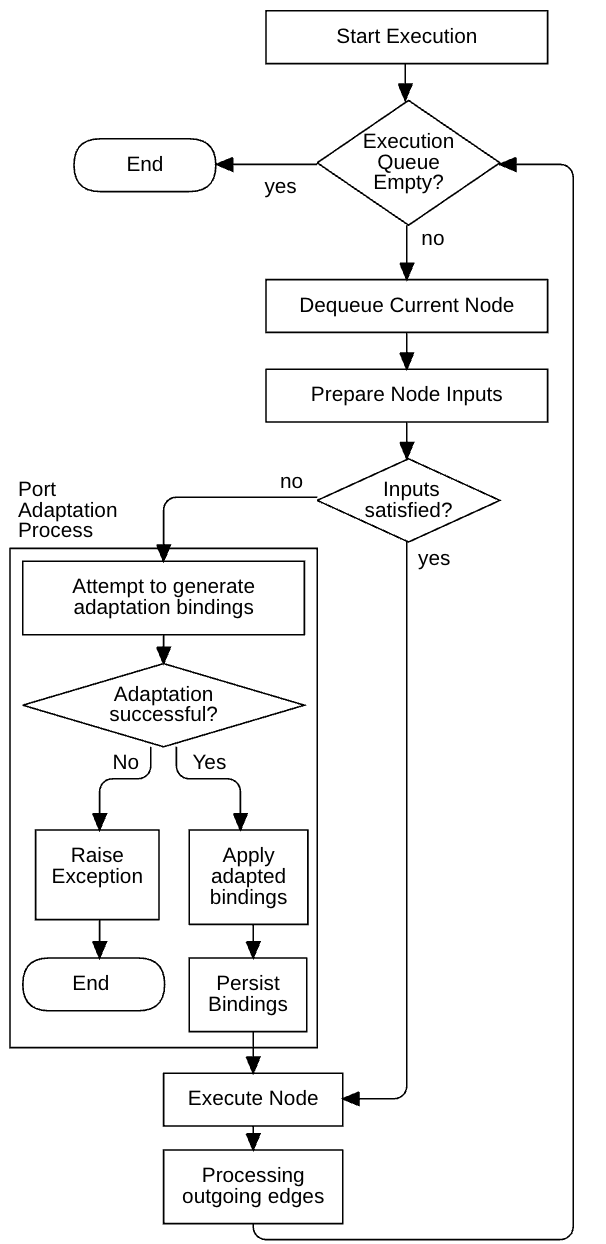
\includegraphics[width=.45\textwidth]{Template_tesi/img/adaption.png}
    \caption{Flowchart of the workflow nodes execution process, detailing the dynamic port adaptation process.}
    \label{fig:adaption-flow-chart} 
\end{figure}


\subsubsection{Workflow Synthesis}


The true potential of this architecture and the SBOM becomes apparent when during the \textit{Workflow Retrieval} phase (Step 3) no pre-assembled workflow capable of handling the user’s intent is found in the Knowledge Base. In such cases, the system can leverage \textit{SBOM-like information} in the Knowledge Layer, which becomes central to the process. This enables the dynamic construction of new workflows by intelligently combining existing nodes. 

Each node is associated with both qualitative and quantitative descriptors—structured and unstructured—which describe its functionality and specifications. These descriptors are embedded and indexed to support \textbf{Hybrid Search}\footnote{An information retrieval method that combines semantic search with full-text search, merging results using algorithms such as Reciprocal Rank Fusion to improve relevance.}, allowing an LLM agent to retrieve and compose components based on their declared capabilities.

This mechanism enables the system to generate workflows that meet \textbf{previously unanticipated requirements}. For instance, if the intent introduces a new constraint, such as a specific latency threshold, the system can construct a workflow by including only nodes whose descriptors indicate compatibility with that latency requirement. Similarly, this applies to verifying the legal compliance or certification status of nodes and tools. Moreover, this mechanism fosters interoperability between vendors, overcoming the major challenges related to the \textbf{lack of standardization} in SBOMs and AIBOMs. Even without a shared or predefined standard or grammar for tracking node dependencies and specifications, considering that different providers may disclose only partial data or use varying formats, an AI-driven approach can transcend these limitations.





Once a suitable workflow is synthesized, it can be saved in the Knowledge Base for future retrieval and reuse. New workflows can be evaluated using established methods such as AI-based judgment, human evaluation, or \textbf{consensus-based voting}. In the latter, multiple agents specialized in workflow construction independently generate candidate workflows, and a workflow is accepted only if it is produced by a majority of agents.

While this high-level approach is promising and underscores the importance of the meta-model repository, further research is required to formalize and systematically structure the process of automatic workflow synthesis.












\subsection{Runtime Adaptations}

As previously discussed, a central advantage of the Reflection pattern is its support for runtime adaptability. In the proposed architecture, agents both retrieve and modify knowledge during execution to accommodate modifications in the environment, dependency structures, or evolving user requirements.
Operational agents interact with the Knowledge Layer to query or update system knowledge in response to runtime conditions. These updates may originate \textbf{externally}—such as from software releases, dependency upgrades, or the introduction of new meta-models—or be \textbf{triggered internally} by components (e.g., the \texttt{Port Adapter Service}; see Section \ref{sec:bindings}) or by system processes (e.g., the generation of new intents and workflows; see \textit{Workflow Execution}, Section \ref{sec:execution}).
To ensure synchronization and consistency between the operational level and the Knowledge Layer, meta-model changes are propagated as events. These events, dispatched via the Meta-Object Protocol (MOP), are received by subscribed operational components, which then adapt their configurations accordingly (see Figure \ref{fig:node-update-event}).


\begin{figure}[h]
    \centering
    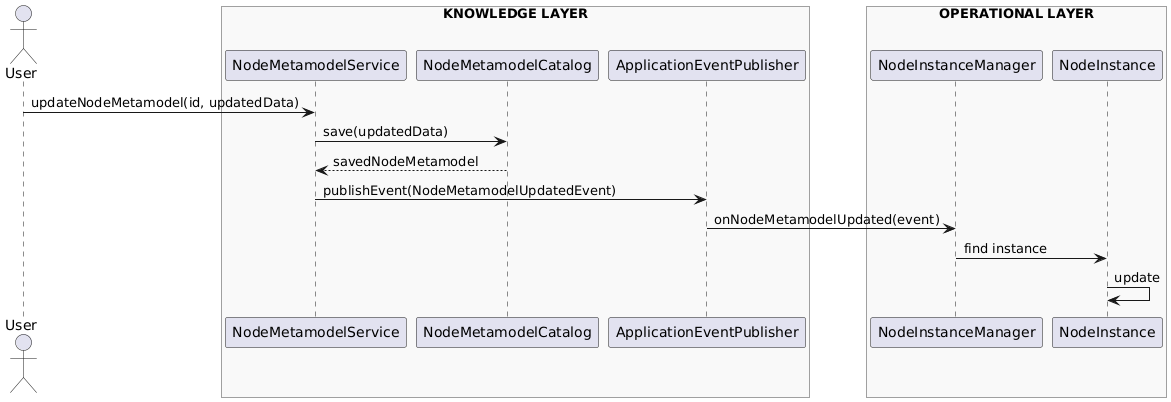
\includegraphics[width=1\textwidth]{Template_tesi/img/node-update-event.png}
    \caption{Propagation of meta-model updates from the Knowledge Layer to operational components via the MOP.}
    \label{fig:node-update-event} 
\end{figure}


\subsubsection{Meta-models Versioning}
In the proposed implementation, the versioning of meta-model catalogs follows the Semantic Versioning\footnote{A versioning scheme that uses the format \texttt{MAJOR.MINOR.PATCH} to indicate the type and impact of changes.} standard.


\begin{itemize}[leftmargin=*, label=--] 
    \item Minor and patch version changes are applied in place within the existing document.
    \item Major version changes (i.e., breaking updates) result in the creation of a new meta-model entry within the catalog.

\end{itemize}



\noindent
Therefore, each meta-model is identified by a unique ID and a family ID, which groups all versions belonging to the same logical component. Within a workflow, nodes reference a specific version of a node.






\subsubsection{Strategies for Instance Updates}
Two primary operational update strategies are employed depending on the nature of the meta-model change:


\begin{itemize}[leftmargin=*, label=--] 
    \item \textbf{Hot-Swapping}: For non-breaking updates, if the instance is not currently running, the system may swap the meta-model in place, seamlessly refreshing the instance.
    \item \textbf{Re-instantiation}: In cases where the instance is currently active or the update constitutes a breaking change (e.g., altered node dependencies in a workflow), the affected meta-model is marked as deprecated. Any future execution of such instances requires a complete re-creation, even if it was previously persisted in the registry.
\end{itemize}








\chapter{Relevant Use Cases: The AI4NE and NE4AI Scenarios}\label{ch:chapter3}

To validate the system's capabilities, this chapter presents an experiment conducted in a network engineering context. The chapter is organized as follows: Section \ref{sec:AI4NE_statement} outlines the problem statement; Section \ref{sec:AI4NE_exp} describes the experimental setup; Section \ref{sec:AI4NE_res} presents the experimental results and concludes with final considerations.


\section{Problem Statement}\label{sec:AI4NE_statement}

Contemporary distributed computing environments are increasingly characterized by heterogeneous hardware resources and dynamically varying network conditions. At the same time, AI workloads demand precise resource allocation to meet requirements related to performance, cost, and compliance. Accordingly, a representative use case integrating both AI for Networking (AI4NE) and Networking for AI (NE4AI) paradigms has been developed to demonstrate the proposed methodology in practice:

\begin{itemize}[leftmargin=*, label=--]
    \item \textbf{AI for Networking} (AI4NE): employing AI models to support routing decisions.
    \item \textbf{Networking for AI} (NE4AI): using the capabilities of programmable networks to optimize the execution and deployment of AI tasks.
\end{itemize}


The overarching goal is to create an intelligent system capable of interpreting user intent, analyzing infrastructure constraints, and routing user tasks across different nodes (or cloud resources), relying on specialized AI modules to optimize networking decisions.

A key advantage of employing an LLM-based methodology is its inherent cross-vendor compatibility, as it supports task specifications and resource requirements expressed in natural language or semi-structured formats, thereby abstracting away vendor-specific dependencies. Furthermore, this method enables \textbf{zero-touch network}\footnote{A self-managing, intent-driven network architecture that automates operations to reduce human error. See Koley, B. The Zero Touch Network, Google Research.} configuration capabilities, allowing network nodes to be dynamically integrated into the distributed topology through automated capability discovery. New nodes are incorporated into the network fabric by providing only their technical specifications and operational manuals, which LLMs then retrieve and process.

\section{Experimental Setup and Feasibility Study}\label{sec:AI4NE_exp}

As an initial feasibility study, preliminary experimentation was conducted to evaluate the viability of the proposed approach. A simplified network abstraction was defined using the following components:

\begin{itemize}[leftmargin=*, label=--]
    \item Hardware Devices: A JSON file containing network device inventories with device identifiers, metadata, and embedded technical manuals extracted from PDF sources with minimal pre-processing.
    \item Network Topology: Encoded as a JSON structure linking each topology node to the corresponding hardware device via unique identifiers.
\end{itemize}


\subsection{Analyzed Approaches}

We examined four distinct approaches to solving the proposed use case.

\subsubsection{Simple LLM}
The first and most naive approach involves a single LLM that processes the entire task by receiving all necessary information in context. This approach is limited by the model's maximum context length, which restricts the amount of input it can handle, as well as the model's internal capabilities. In this setting, the LLM was prompted to directly produce the final answer, along with a motivation for the main decisions involved in the process.

\subsubsection{Reasoning LLM}
This approach is similar to the simple LLM setup but incorporates a structured reasoning process. The prompt was modified to explicitly request a step-by-step explanation using the Chain-of-Thought (CoT) prompting technique. A reasoning template was provided to guide the model through the intermediate steps required to reach the final decision.

\subsubsection{Function Calling }
A way to significantly improve the model's functionality and integrate it with real-world systems and external data sources is the Function Calling technique. Function Calling—referred to as Tool Calling in Spring AI—is a mechanism that enables LLMs to invoke external functions. Beyond generating textual responses, the model can autonomously determine whether and when to call predefined APIs or services (defined as tools) to gather accurate data or perform actions.

\subsubsection{Cognitive Workflow }
Finally, we evaluated our implementation of a Cognitive Workflow. Cognitive Workflows formalize the Chain-of-Agents pattern (also known as Prompt Chaining \cite{schluntz2024building} or Chain Workflow \cite{tzolov2025agentic}). As noted by the Spring Blog, this structure is suitable for tasks with clearly defined, sequential steps, balancing latency and accuracy. Unlike agent planners—such as the Plan-and-Execute pattern used in frameworks like LangChain (see Appendix \ref{ch:appendix_spring})—which separate planning and execution at runtime, the cognitive workflow engine executes a structured sequence of nodes representing the task decomposition. Although workflows can be synthesized dynamically or retrieved from a meta-model catalog, their structure is fixed upon instantiation, eliminating the need for runtime planning.

We argue that this design enhances functional sustainability, reliability (key ISO/IEC 25010 quality attributes), and explainability.



\subsection{Workflow Design}
A preliminary workflow was designed for the AI4NE and NE4AI scenarios. The task was decomposed into five steps:




\begin{enumerate}
    \item \textbf{Intent Detection and Requirement Extraction} (LLM): The system's core LLM agent infers the user's intent and desired service, extracting a structured list of requirements.
    
    \item \textbf{Hardware Retrieval} (Tool): An external tool retrieves the list of hardware devices currently available in the network.
    
    \item \textbf{Hardware Selection} (LLM): Based on the technical manuals, the LLM selects candidate devices that meet the functional requirements. This agent has no awareness of the network topology.
    
    \item \textbf{Routing Computation} (Tool): A topology-aware tool computes possible routes from the source to the target node, ensuring that at least one candidate device is included in each path. Traditional algorithms, such as Dijkstra's and K-Shortest Paths (KSP), are used.
    
    \item \textbf{Route Finalization} (LLM): A final LLM agent receives the candidate paths and, based on the previously defined requirements, selects the optimal route.
    
    \end{enumerate}
    


The separation of hardware selection and routing computation is key. The LLM responsible for hardware selection operates independently of network topology, reducing complexity by avoiding the need to consider all potential (exponentially many) source-to-target paths. Instead, hardware capabilities serve as a heuristic for narrowing the search space early in the process.

Additionally, this hybrid design, involving early candidate discovery followed by routing optimization and finalization, is conceptually aligned with existing research in AI-driven SDN\footnote{Software-Defined Networking} control. For example, Guo and Yuan \cite{guo2021network} proposed a similar architecture, though based on traditional machine learning (ML) techniques rather than large language models (LLMs). Their approach involves generating multiple candidate routing paths using classical algorithms such as Dijkstra and K-Shortest Path (KSP). These paths are then evaluated and optimized through ML-based techniques, including genetic algorithms, particle swarm optimization, and simulated annealing, all operating under multi-objective criteria. Once an optimal routing strategy is identified, it is enforced by the SDN controller, which dynamically reconfigures the network. 


\subsection{Comparative Implementation Approaches}
Regarding the Function Calling approach, all services utilized in the workflow definition, as well as an additional endpoint for retrieving network topology, were made available to the model through the Spring AI function calling implementation.

In contrast, for the simple LLM approach, the devices and network information were retrieved prior to the LLM invocation, and the system prompt was augmented with all the necessary information to process the request. The routing service was not used in this configuration; therefore, routing became the sole responsibility of the LLM through a direct analysis of the topology structure.


\section{Empirical Results and Analysis}\label{sec:AI4NE_res}

In the initial network configuration, we deployed a simplified prototype of a software-defined network (SDN) composed of five interconnected nodes, including two AI-capable devices. A diverse suite of test workloads was submitted to the four systems, encompassing both AI-oriented tasks—ranging from lightweight inference jobs to computationally demanding training operations—and non-AI scenarios requiring advanced networking capabilities. The latter included ultra-low-latency trading connections, 5G-Advanced communication, and hardware-accelerated packet processing. The evaluation focused on three main dimensions:

\begin{itemize}[leftmargin=*, label=--]
\item Feasibility and correctness of the computed network paths.
\item Determinism and consistency of the path computation when provided with identical or slightly varied prompts.
\item Average planning time required for routing.
\end{itemize}

Multiple tests were performed, but only the most noteworthy results are reported here.

To begin, we evaluated a routing scenario involving AI-enhanced signal processing across the four systems over 20 iterations using a consistent prompt (see Figure~\ref{fig:test1a}). The Cognitive Workflow and Reasoning LLM approaches demonstrated the highest reliability, followed by the Function Calling method, and lastly the Simple LLM. However, this reliability came at a performance cost: both the Cognitive Workflow and the Reasoning LLM incurred significant execution overhead. On average, the Simple LLM was 49\% faster than the Cognitive Workflow, while the Function Calling method was 30\% faster.

\begin{figure}[h]
\centering
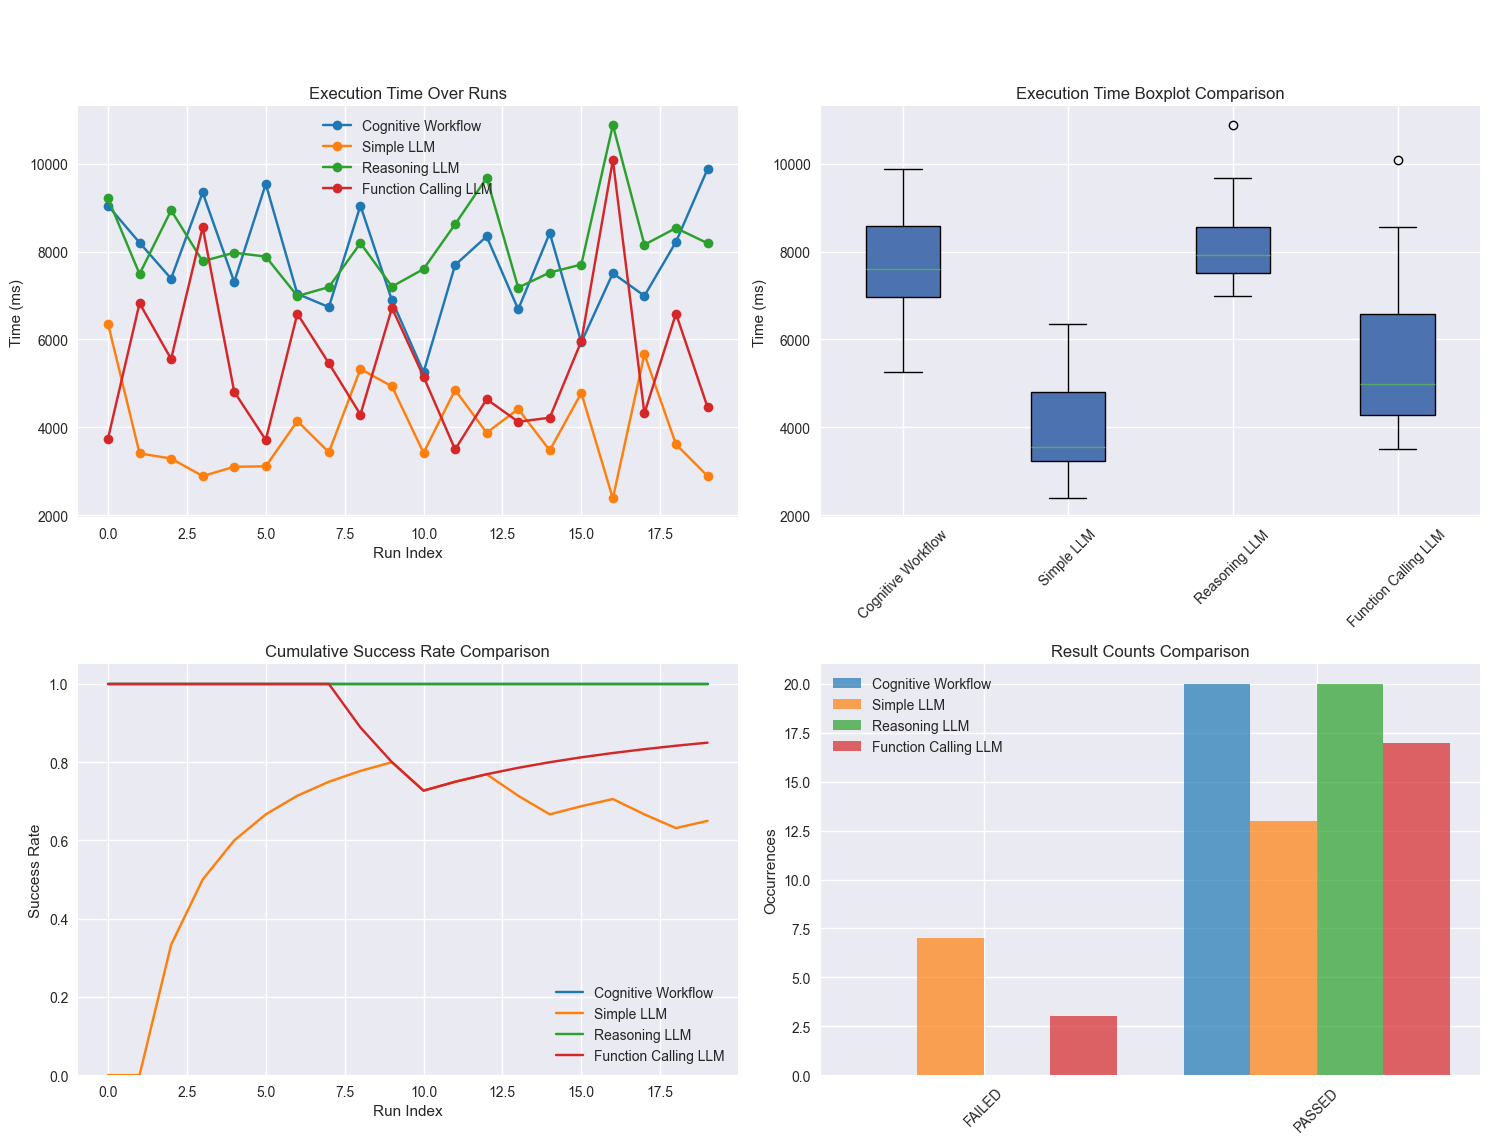
\includegraphics[width=1\textwidth]{Template_tesi/img/a4ne/1a.png}
\caption{Performance and reliability comparison of the four approaches under a 5G network routing scenario involving AI-enhanced signal processing.}
\label{fig:test1a}
\end{figure}


Another interesting and more challenging test case involved the same network, where the following configuration was requested:

\begin{promptboxcontent}
\small\textit{Configure a high-throughput network to process sensor fusion data from 500 Google Waymo autonomous vehicles for centralized AI training. Each vehicle streams 80 MB/s of LiDAR, camera, and radar data. A single processing node must ingest all incoming data streams, utilizing NVMe-over-Fabrics storage for training dataset ingestion and hardware-accelerated preprocessing before forwarding the data to downstream GPU training clusters.}
\end{promptboxcontent}
%\promptcaption{pr:network_config}{High‑Throughput Network Configuration Request}

This prompt is more demanding than the previous one. Rather than relying on basic feature matching from device manuals for hardware selection, it required mathematical reasoning to compute the total requested workload. Specifically, it was necessary to aggregate the input data rate as follows:

\begin{align*}
\text{Data rate per vehicle} &= 80~\text{MB/s} = 0.64~\text{Gb/s} \\
\text{Total for 500 vehicles} &= 500 \times 0.64 = 320~\text{Gb/s} \\
\text{With a requested 5\% margin} &= 320 \times 1.05 = \boxed{336~\text{Gb/s}}
\end{align*}

\noindent
This made the test unambiguous, since only one device, namely the NVIDIA BlueField-3 DPU, could meet the required throughput (up to 400 Gb/s).


\begin{figure}[h]
    \centering
    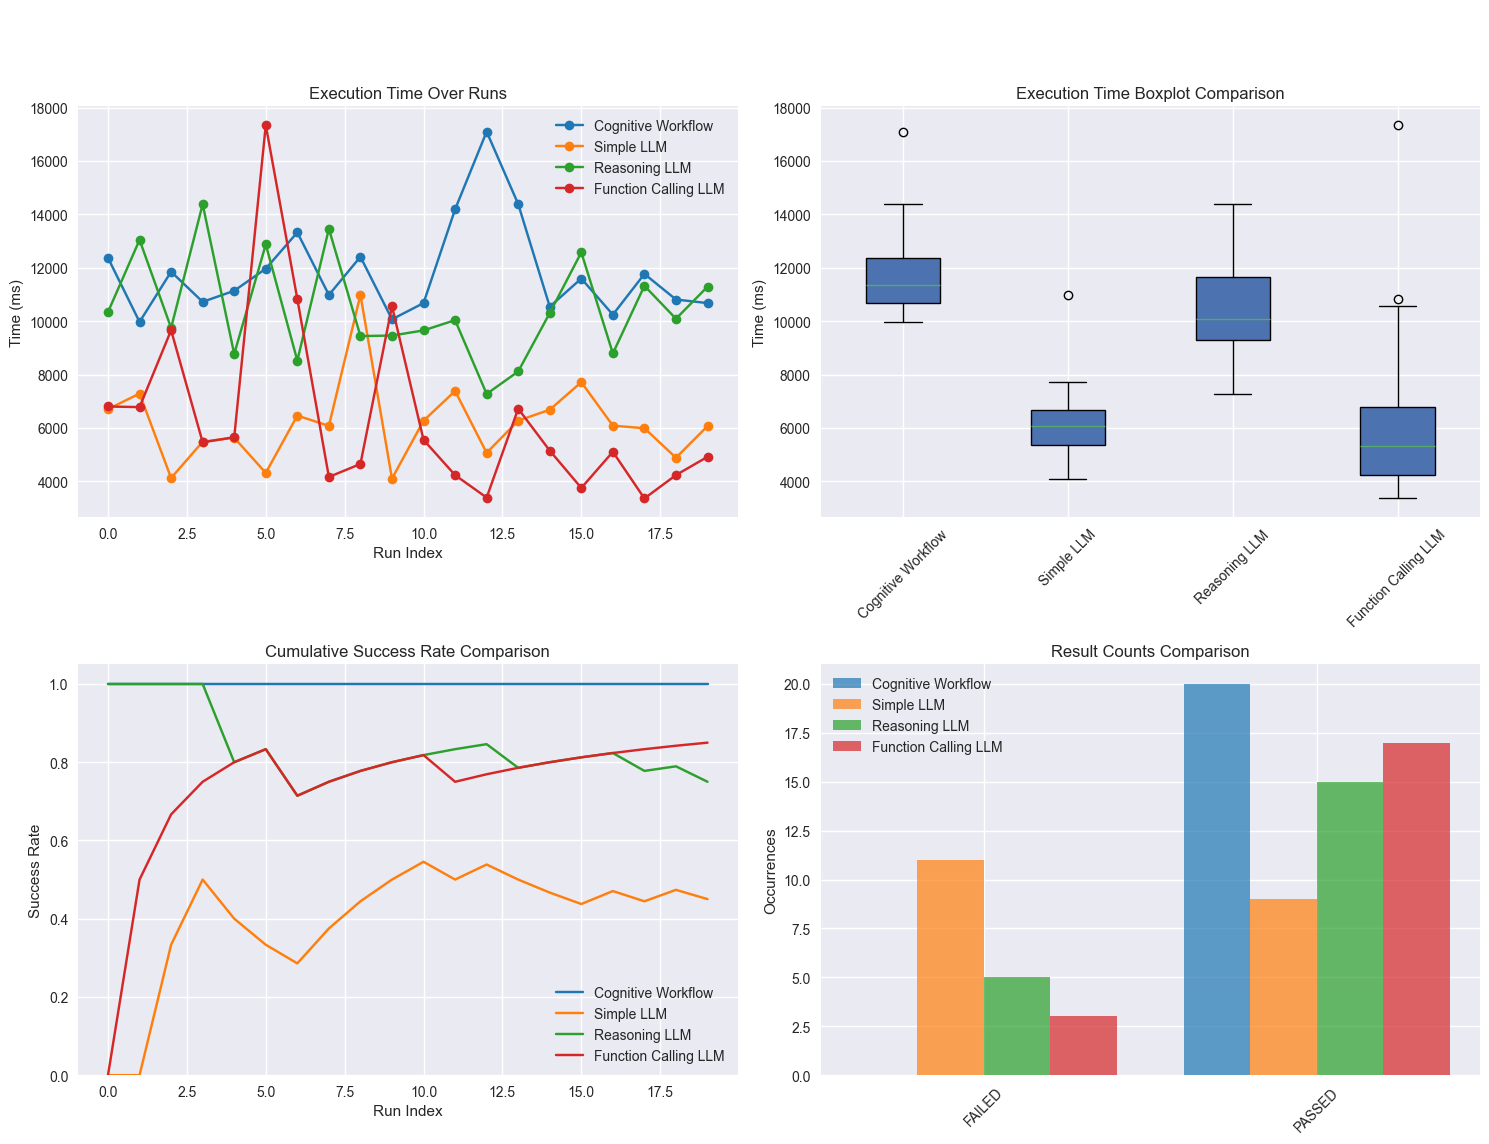
\includegraphics[width=1\textwidth]{Template_tesi/img/a4ne/1b.png}
    \caption{Performance and reliability comparison of the four approaches processing a complex network configuration scenario that requires aggregating multiple specifications and performing throughput calculations.}
    \label{fig:test1b} 
\end{figure}


In this scenario, the Cognitive Workflow once again achieved the highest accuracy, followed by the Function Calling agent. The Reasoning LLM, even without external tools, demonstrated a remarkable accuracy comparable to that of the Function Calling agent, though it was significantly slower. The Simple LLM, by contrast, had a success rate below 50\% (see Figure~\ref{fig:test1b}). 




\begin{figure}[h]
    \centering
    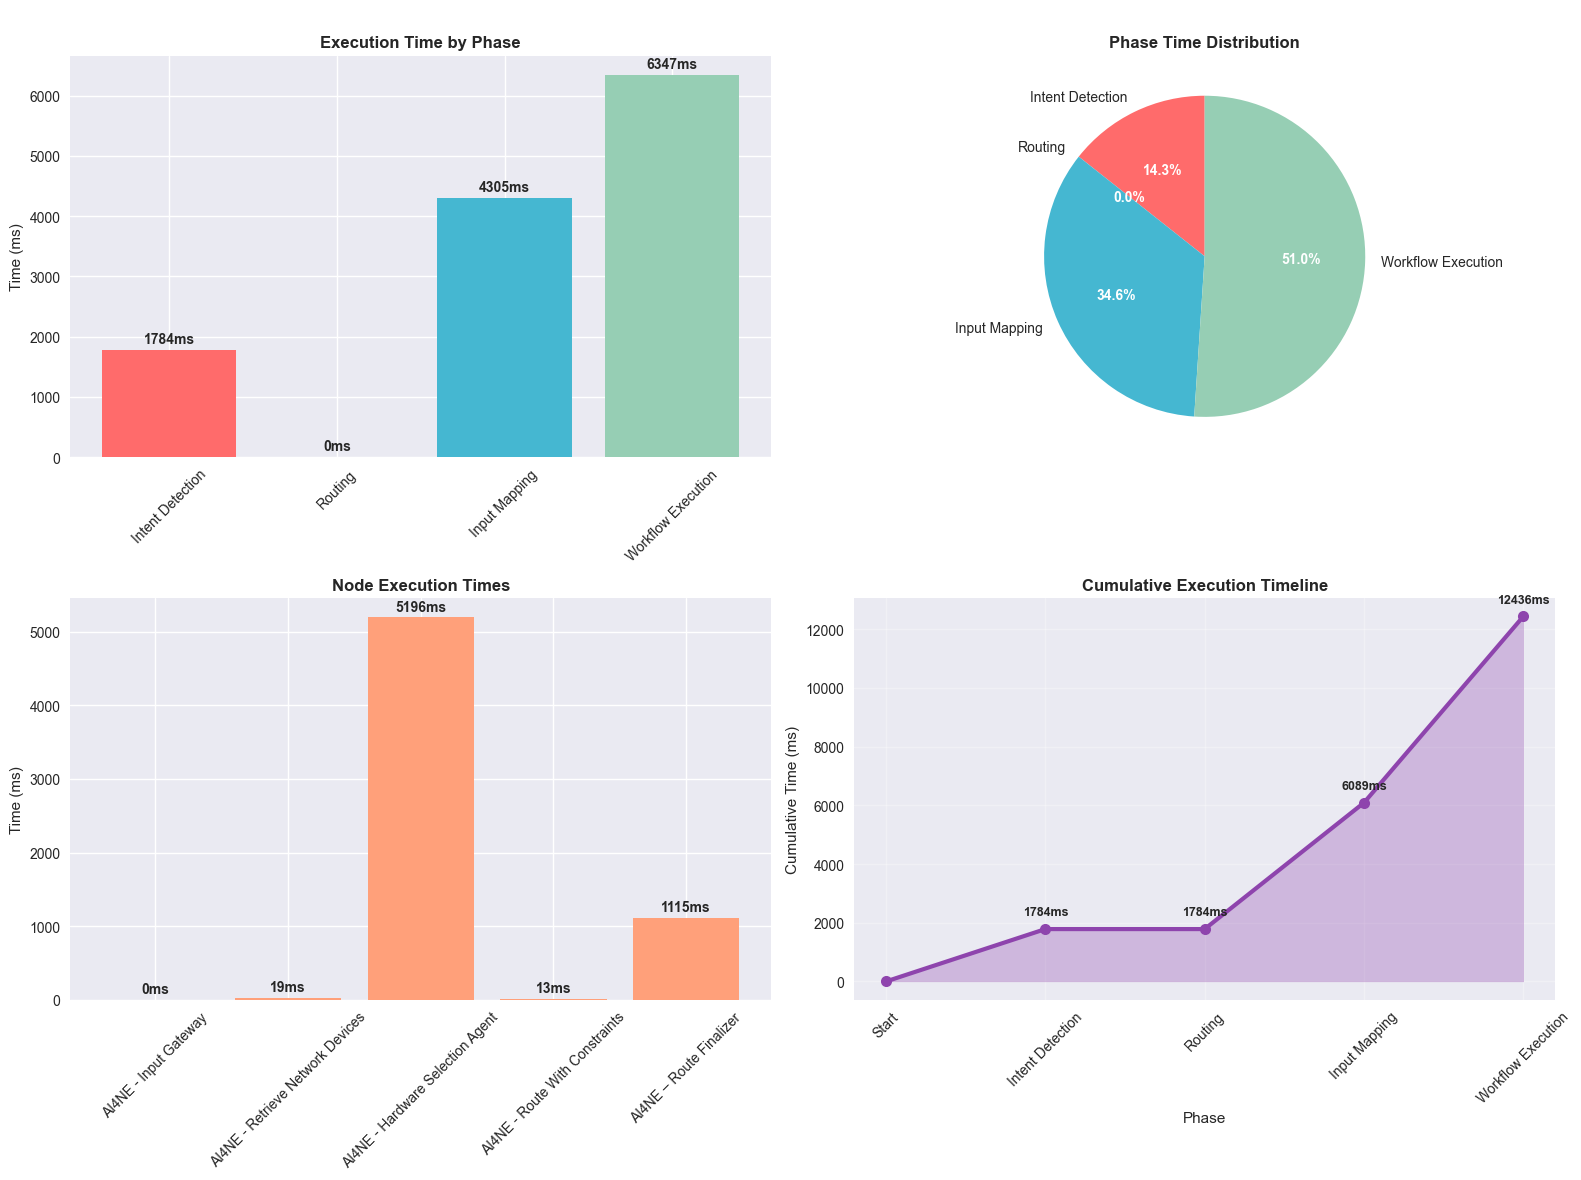
\includegraphics[width=1\textwidth]{Template_tesi/img/a4ne/observability.png}
    \caption{Execution time breakdown of a Cognitive Workflow, detailing phases including intent detection, input mapping, and subsequent processing steps.}
    \label{fig:time-breakdown} 
\end{figure}


Interestingly, execution times increased across all methods, particularly for the Cognitive Workflow. This was likely due to the mathematical reasoning required by the task, as well as, in the case of the Cognitive Workflow, the greater number of constraints expressed in the prompt—which extended both the intent detection and input mapping phases. The execution time breakdowns (Figure \ref{fig:time-breakdown}) support this observation: approximately 34.6\% of the total execution time was spent on input mapping, which took about 31.4\% more time in absolute terms compared to the first test scenario. Additionally, 14.3\% of the time was spent on intent detection, which introduced unnecessary overhead, given that only a single intent was involved. While these results highlight structural trade-offs between the two approaches, performance can still be improved through targeted optimizations, such as using smaller foundational models, applying prompt engineering techniques, and implementing caching strategies (see Section \ref{sec:next_steps}).




\subsection{Observations}
During the evaluation of the four approaches, we observed recurring patterns that offer critical insights:


\begin{itemize}[leftmargin=*, label=--]
\item \textbf{Tool Calling Inconsistency}: The function-calling setup exhibited inconsistencies in the execution of tools. Despite clear, step-by-step instructions and tool definitions, the system occasionally deviated from the expected flow—invoking tools out of order. For instance, it sometimes bypassed the routing tool entirely and attempted path selection autonomously, undermining the intended separation between reasoning and computation. In other cases, the same tools were invoked multiple times, resulting in unnecessary delays in execution.

\item \textbf{Self-Explanation Prompting}: All agents showed improved performance when prompted to justify their decisions, although this was accompanied by increased token usage. Notably, the single LLM variant, when not required to generate explicit explanations, frequently failed even on simple tasks. Instructing for motivations regarding the inclusion or exclusion of hardware devices also enhanced the accuracy of the Hardware Selector Node within the Cognitive Workflow.

\item \textbf{Chain-of-Thought Prompting}: Failures observed in the single-LLM setup were often not due to flawed logic or incorrect decision criteria but rather to incomplete or invalid output paths, even with self-explanation prompting. In several instances, paths were missing critical intermediate nodes, or the model incorrectly assumed the existence of edges not present in the actual topology. In other cases, the model failed to associate device identifiers with corresponding node identifiers properly. When the agent was guided to apply the Chain-of-Thought (CoT) prompting technique—breaking down the task into a series of reasoning steps, including hardware evaluation for each device, enumeration of connecting edges, and validation of the entire path—these topology-related errors were largely resolved. 

\item \textbf{Self-Contradiction}: Both the Simple LLM and the Function Calling agent occasionally produced outputs where the reasoning did not align with the final path selected. In several cases, the explanation referenced a combination of multiple selected devices, while the final result included only a single device. These inconsistencies suggest difficulties in maintaining coherent reasoning under complex, multi-constraint scenarios—especially when operating near token limits.


\end{itemize}

Additional implementation challenges for the Cognitive Workflow are discussed in Section \ref{sec:challenge}.



\subsection{Key Insights and Future Directions}


Several important insights and future considerations were revealed during the evaluation experiment:

\begin{itemize}[leftmargin=*, label=--]

  \item \textbf{Necessity of a more challenging evaluation framework}: The unexpectedly strong performance of the simple LLM in early tasks suggests that the test environment may be too simplistic to highlight the benefits of structured workflows effectively. A more demanding testbed should include:
    \begin{itemize}[leftmargin=2em, label=--]
      \item Network topologies that are too complex for an LLM to solve unaided, including multi-layered networks with compute and switch devices.
      \item Weighted graphs that accurately reflect real-world constraints, including latency and bandwidth.
      \item Greater device heterogeneity and volume to surpass the context limit of a single LLM.
    \end{itemize}

  \item \textbf{Improving Task Clarity}: A recurring challenge was formulating tasks that were both non-trivial and unambiguous. Although the tasks were designed to require multidimensional reasoning, we frequently encountered ambiguity in hardware selection, which compromised reproducibility. This was often due to under-specified constraints or vague prompt formulations. To address this, we propose formalizing natural language requests and qualitative attributes into structured, quantitative requirement vectors by estimating hardware requirements prior to hardware selection (e.g., minimum TFLOPS $\geq$ 15, maximum latency $\leq$ 20 ms, etc.). This approach may reduce the incidence of multiple equally plausible solutions.

\end{itemize}


\subsection{Conclusion}
This feasibility study demonstrates that LLMs when embedded within cognitive workflow architectures, can support complex decision-making processes—while also exposing significant limitations. Although the networking scenario served as a valuable practical demonstration, it is not intended as a comprehensive exploration of the domain. Nonetheless, these initial findings encourage deeper investigation  on LLM-based cognitive systems in both AI for Network Engineering (AI4NE) and Network Engineering for AI (NE4AI) contexts.


\chapter{Discussion and Future Work}\label{ch:chapter4}

This final chapter presents a discussion of the proposed architecture's outcomes and explores its implications, limitations, and future evolution. Section \ref{sec:challenge} examines the key challenges encountered during development and the limits of the present implementation; Section \ref{sec:next_steps} outlines future research directions; finally, Section \ref{sec:conclusion} presents our concluding observations on the contribution of this work.


\section{Challenges} \label{sec:challenge}

The implementation of the proposed framework brought to light several challenges, which can be broadly categorized as architectural limitations of the framework and difficulties encountered during development.



\subsection{Framework Complexities and Limitations}


\subsubsection{Performance Overhead}
The integration of meta-model catalogs introduced a measurable performance overhead compared to traditional approaches. The necessity to query and update meta-information at runtime, along with validating component compatibility, led to increased latency in workflow execution, as demonstrated by the controlled experiments illustrated in Chapter \ref{ch:chapter3}.
This overhead is notably pronounced during the starting phases of workflow execution, where intent detection, variable extraction and mapping, and compatibility validation must occur before the actual processing begins. 
While this performance bottleneck might be a concern in some latency-critical applications, it could be acceptable given the improved transparency, adaptability, and—most importantly—reliability, as demonstrated by the experiments.


\subsubsection{Complexity of Meta-Information Management}
One of the most notable challenges encountered was maintaining accurate and up-to-date metadata across the system. As the number of nodes and their interdependencies grew, the complexity of tracking configuration updates became substantial. Furthermore, the heterogeneous nature of AI components exacerbates this challenge. Different model providers use varying metadata and configuration formats, making it challenging to define an abstract schema that is suitable for all LLM providers.

\subsubsection{State Consistency}
The dual-layer architecture presents new challenges related to state consistency. For example, when workflows depend on nodes that are subjected to breaking changes, the system cannot automatically attempt to adapt. Similarly, the situation in which a workflow is running while the nodes are updated concurrently requires better management and is a subject of future inquiry. Such divergences can lead to decisions based on outdated or incomplete information, which can compromise reliability.

\subsubsection{Domain Precision}
A key complexity of the framework lies in configuring the system and meta-information to operate with fine granularity across diverse domains. Aiming for an out-of-the-box, highly adaptable system risks losing precision in specific applications. This issue was evident during the setup of the AI4NE/NE4AI experiments (Chapter \ref{ch:chapter3}). For example, the system's intent detector failed to recognize certain specialized operations as refinements of broader intent categories, suggesting the need for additional domain-specific knowledge. Similarly, variable extraction poses domain-dependent challenges. In some applications, variables must be extracted with absolute fidelity; in others, conversions or qualitative-to-quantitative mappings are required, while some cases demand intelligent aggregation (without fabricating data). Accordingly, core AI components must be dynamically configured per domain, striking a balance between generalizability and domain-specific precision.


\subsection{Challenges in System Development}

\subsubsection{Tooling Immaturity }
While Spring AI offered a promising foundation for integrating LLM capabilities into Java-based systems, its relative novelty meant that documentation, tooling, and community support were still in the process of evolving. Consequently, several components required custom implementation, and some bugs were encountered—for example, issues with prompt templates and structured outputs failing due to JSON within the prompt, as documented in issue \texttt{\#2836}\footnote{See \url{https://github.com/spring-projects/spring-ai/issues/2836} (Accessed on June 9, 2025)} and issue \texttt{\#2347}\footnote{See \url{https://github.com/spring-projects/spring-ai/issues/2347} (Accessed on June 9, 2025)}.

\subsubsection{Lack of Standardization}
As discussed in Chapter \ref{ch:chapter1}, while the concept of SBOM is relatively mature in traditional software domains, its extension to AI remains unstandardized. This results in ambiguity when defining the scope and schema of the AIBOM, especially concerning components such as LLM configurations, datasets, prompt templates, and inter-agent interactions. Establishing an effective representation therefore required iterative refinement and custom schema design, given the absence of widely adopted best practices.


\subsubsection{Evaluation of LLM-based Components}
Validating the correctness and stability of LLM-powered services proved challenging due to their nondeterministic and open-ended nature. Extensive testing was required to guarantee high reliability, especially for the structured data flow. This involved testing complex, deeply nested adaptations of intricate schemas, as well as ensuring strict compliance with the structured output models. Moreover, guaranteeing consistent behavior across different prompts, providers, and model versions necessitated comprehensive integration testing, which incurred notable costs associated with API usage. For more details, see the testing strategy outlined in Appendix \ref{appendix_details}.



\section{Next steps} \label{sec:next_steps}

This section outlines future directions for refining the framework’s implementation and identifies key research opportunities.


\subsection{Prospects for Implementation Refinement}


\subsubsection{Advanced Workflow Synthesis }

Although the current implementation is designed to support autonomous workflow synthesis, substantial research is still required. Nevertheless, this also opens up significant opportunities for advancement, particularly in the following areas:


\begin{itemize}[leftmargin=*, label=--]
  
    \item\textbf{Workflow Optimization}: Developing a more sophisticated core logic that employs multi-objective optimization techniques could enable the system to balance competing objectives—such as performance, cost, energy efficiency, and regulatory compliance—simultaneously. 

    \item\textbf{Formal Verification Methods}: Although the proposed implementation already features verification services to check the quality of meta-level artifacts, integrating formal verification techniques would further strengthen correctness guarantees. This is especially critical in safety-sensitive domains.
    
    \item\textbf{AI as a Judge}: Introducing an AI-based mechanism to automatically assess both the meta-model structure and execution outputs of workflows is necessary. This would enable the consistent evaluation of both automatically generated and manually crafted workflows, assisting in the detection of regressions and ensuring system reliability. Given the open-ended nature of workflow execution and the absence of an exact ground truth, an LLM agent is particularly well-suited for this task.

\end{itemize}



\subsubsection{Security and Privacy Enhancements}
Future developments should focus on addressing security and privacy, building on the strategies already discussed in the cited works \cite{xia2024trust, barclay2022providing}. To improve accountability, integrating trust mechanisms such as verifiable credentials or blockchain-based audit trails could prove effective. In particular, the secure sharing of SBOM data could rely on techniques such as zero-knowledge proofs \cite{w3c_zkp}, which allow verification of compliance without revealing specific implementation details.



\subsubsection{Enhanced Scalability}
To facilitate enterprise-scale implementations, subsequent efforts should concentrate on:

\begin{itemize}[leftmargin=*, label=--]
\item\textbf{Distributed Architecture}: Evolute from the centralized prototype to a fully distributed system, as outlined in the SALLMA design, to ensure scalability and fault tolerance, while maintaining consistency across meta-models.

\item\textbf{Hierarchical AIBOM Management}: Implement a multi-level AIBOM structure that supports efficient querying and updates at multiple levels of granularity—combining summary-level views for strategic decisions with detailed data for operational analysis.

\item\textbf{Caching Strategy}: Replace in-memory caching with scalable solutions like Redis and introduce prefetching to anticipate metadata needs, reducing latency and improving system responsiveness.
\end{itemize}



\subsection{Directions for Future Research}

To lay the foundation for future developments, this study opens up several promising research directions that aim to validate the proposed approach. 

The first direction involves \textbf{quantitative evaluations} of the system via controlled modifications of the AIBOM. By altering the information in the meta-catalogs, it is possible to assess the system's resilience, sensitivity, and adaptive capabilities. These experiments would yield measurable insights into the robustness of cognitive workflows when faced with changes in component-level descriptors.

A second key direction focuses on \textbf{knowledge subtraction scenarios}. This line of inquiry aims to analyze how the removal or degradation of structured or unstructured knowledge affects the system's behavior. Future investigations could explore the effects of excluding specific nodes, metadata fields, or knowledge base entries from the meta-model, assessing whether the system can compensate for the missing information.




\section{Conclusion} \label{sec:conclusion}
This thesis introduced a two-fold framework that addresses critical gaps in the literature and industry in the domain of multi-agent AI systems. By combining the Reflection architectural pattern with the concept of the AI Bill of Materials, it has been demonstrated how cognitive workflows can achieve enhanced reliability, portability, and maintainability. The convergence of regulatory requirements,  emerging business demands, and existing research gaps offers a timely opportunity for implementing solutions such as the one proposed in this study. As artificial intelligence becomes more integral to critical infrastructure and decision-making processes, robust governance mechanisms become indispensable. 

In conclusion, this research, situated at the intersection of software engineering and AI engineering, offers both theoretical foundations and practical insights for addressing the growing complexity of modern artificial intelligence systems. Looking ahead, the effectiveness of future multi-agent architectures will depend not only on their technical capabilities but also on their traceability, adaptability, and accountability. The presented framework marks a step toward this vision, fostering the development of more trustworthy and resilient AI solutions. As the field continues to mature, such approaches will be essential for securing public trust and ensuring the reliable integration of AI into high-stakes domains.





\appendix

\chapter{Implementation Details and Supplementary Materials}
\label{appendix_details}

This appendix provides additional technical insight to support the implementation described in Chapter \ref{ch:chapter2}.


\section*{UML Diagrams}

This section presents UML diagrams that illustrate the structural design and interrelationships of the system's core components. Figure~\ref{fig:uml_knowledge} depicts the \textbf{Knowledge Layer}, which encapsulates the domain model and the repositories used for Object-Document mapping (ODM). Serving as the backbone, the Meta-Object Protocol (MOP) is realized through five distinct services. These services manage the meta-models and facilitate advanced capabilities such as Hybrid Search.


\begin{figure}
  \centering
  \begin{adjustbox}{center}
    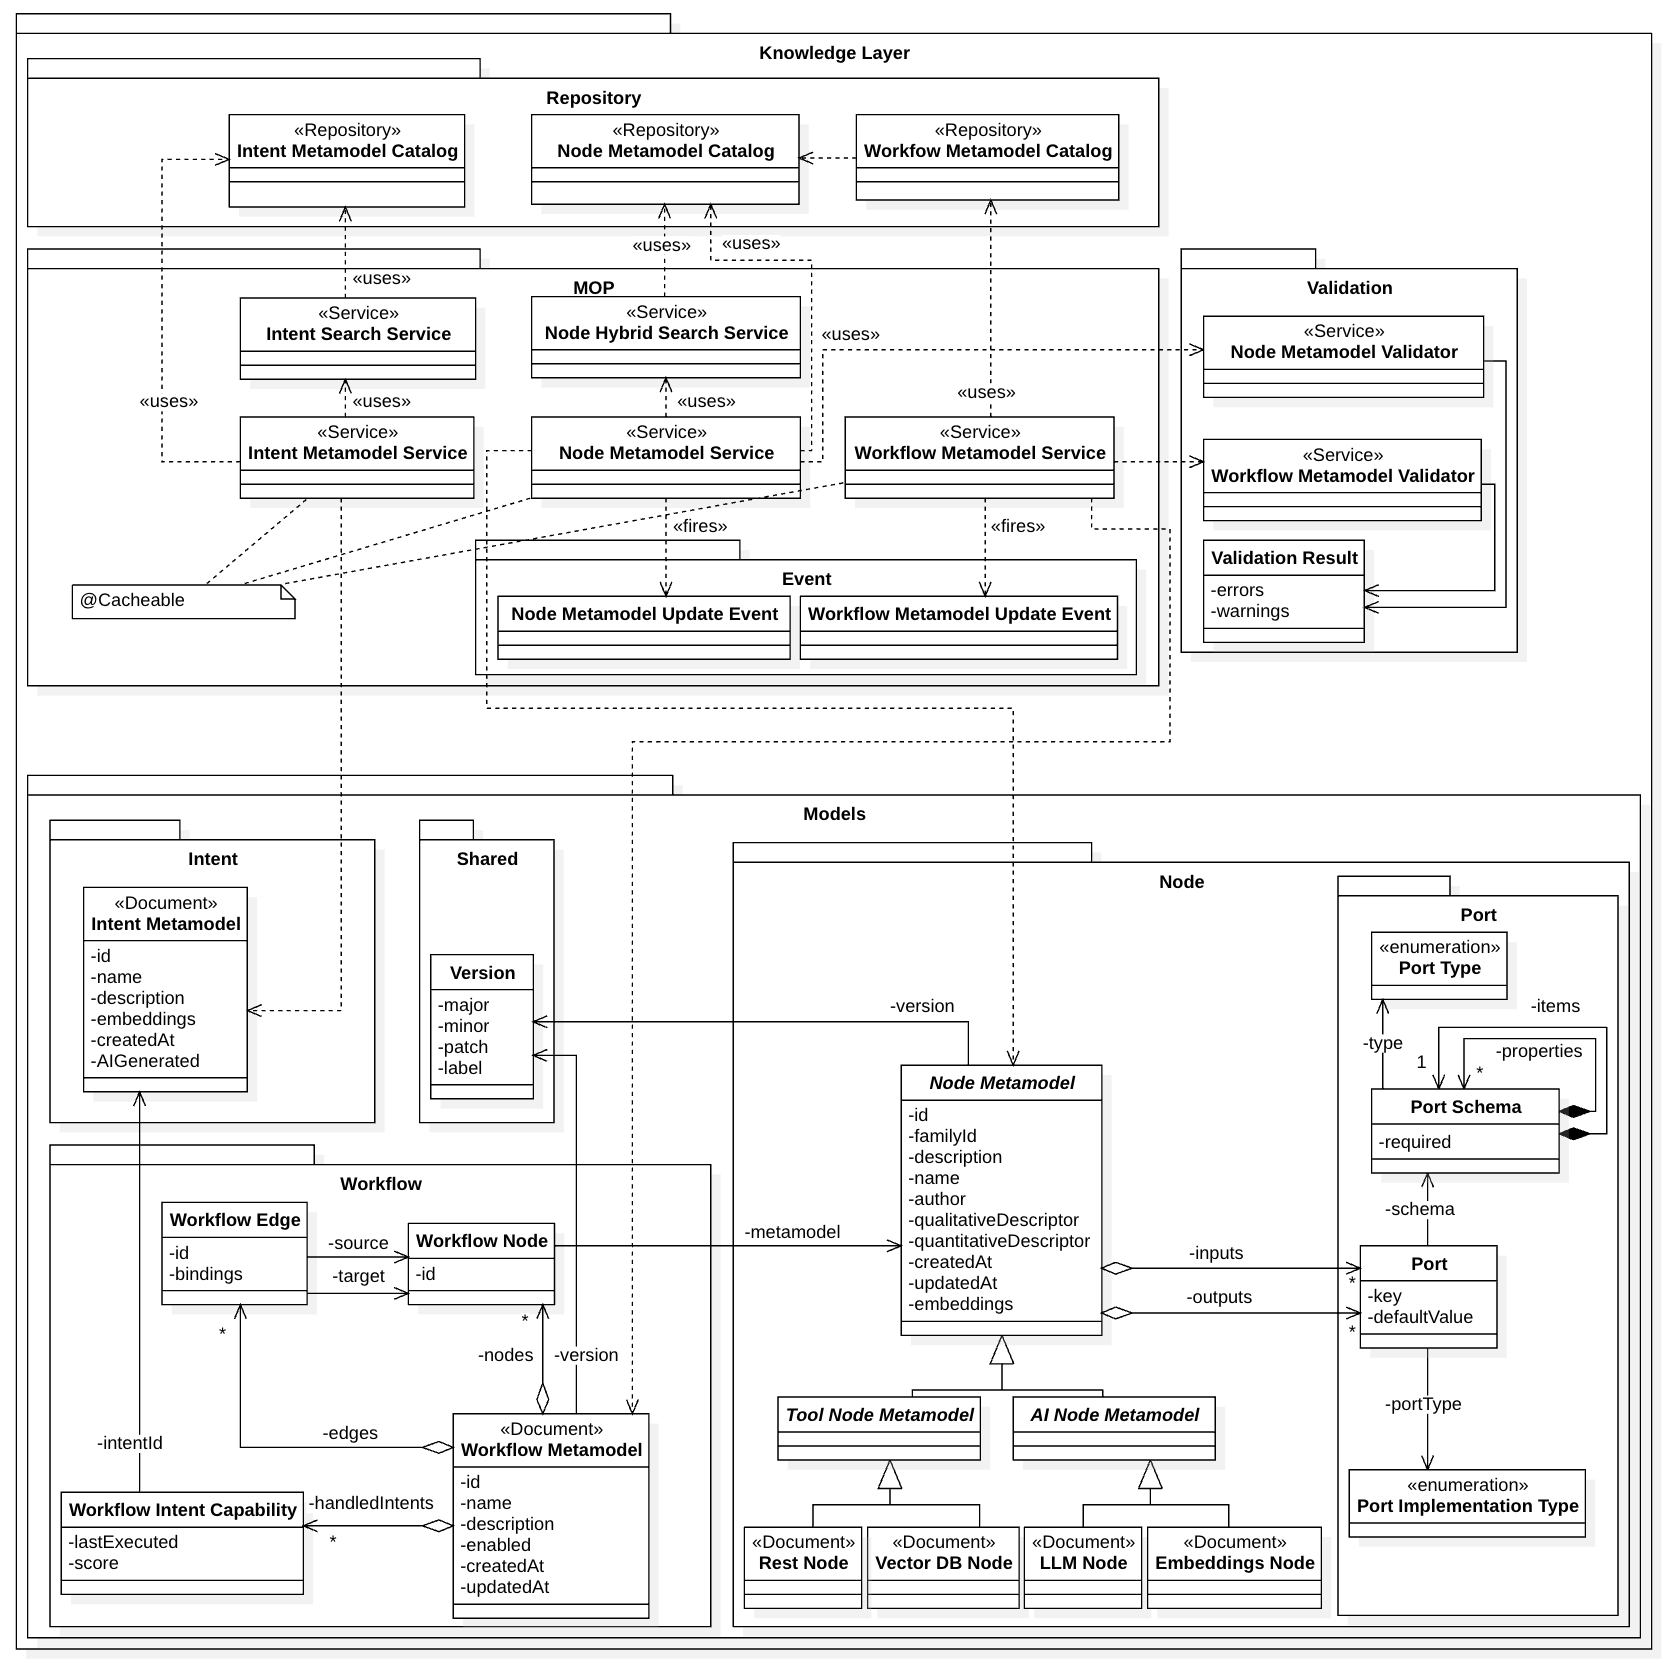
\includegraphics[width=1.2\textwidth]{Template_tesi/img/uml_knowledge.png}
  \end{adjustbox}
    \caption{UML Diagram of the \texttt{knowledge} package, illustrating its internal structure and relationships with other components. For conciseness, standard getters/setters and non-essential elements have been excluded.}
    \label{fig:uml_knowledge}
\end{figure}


\begin{figure}
  \centering
  \begin{adjustbox}{center}
    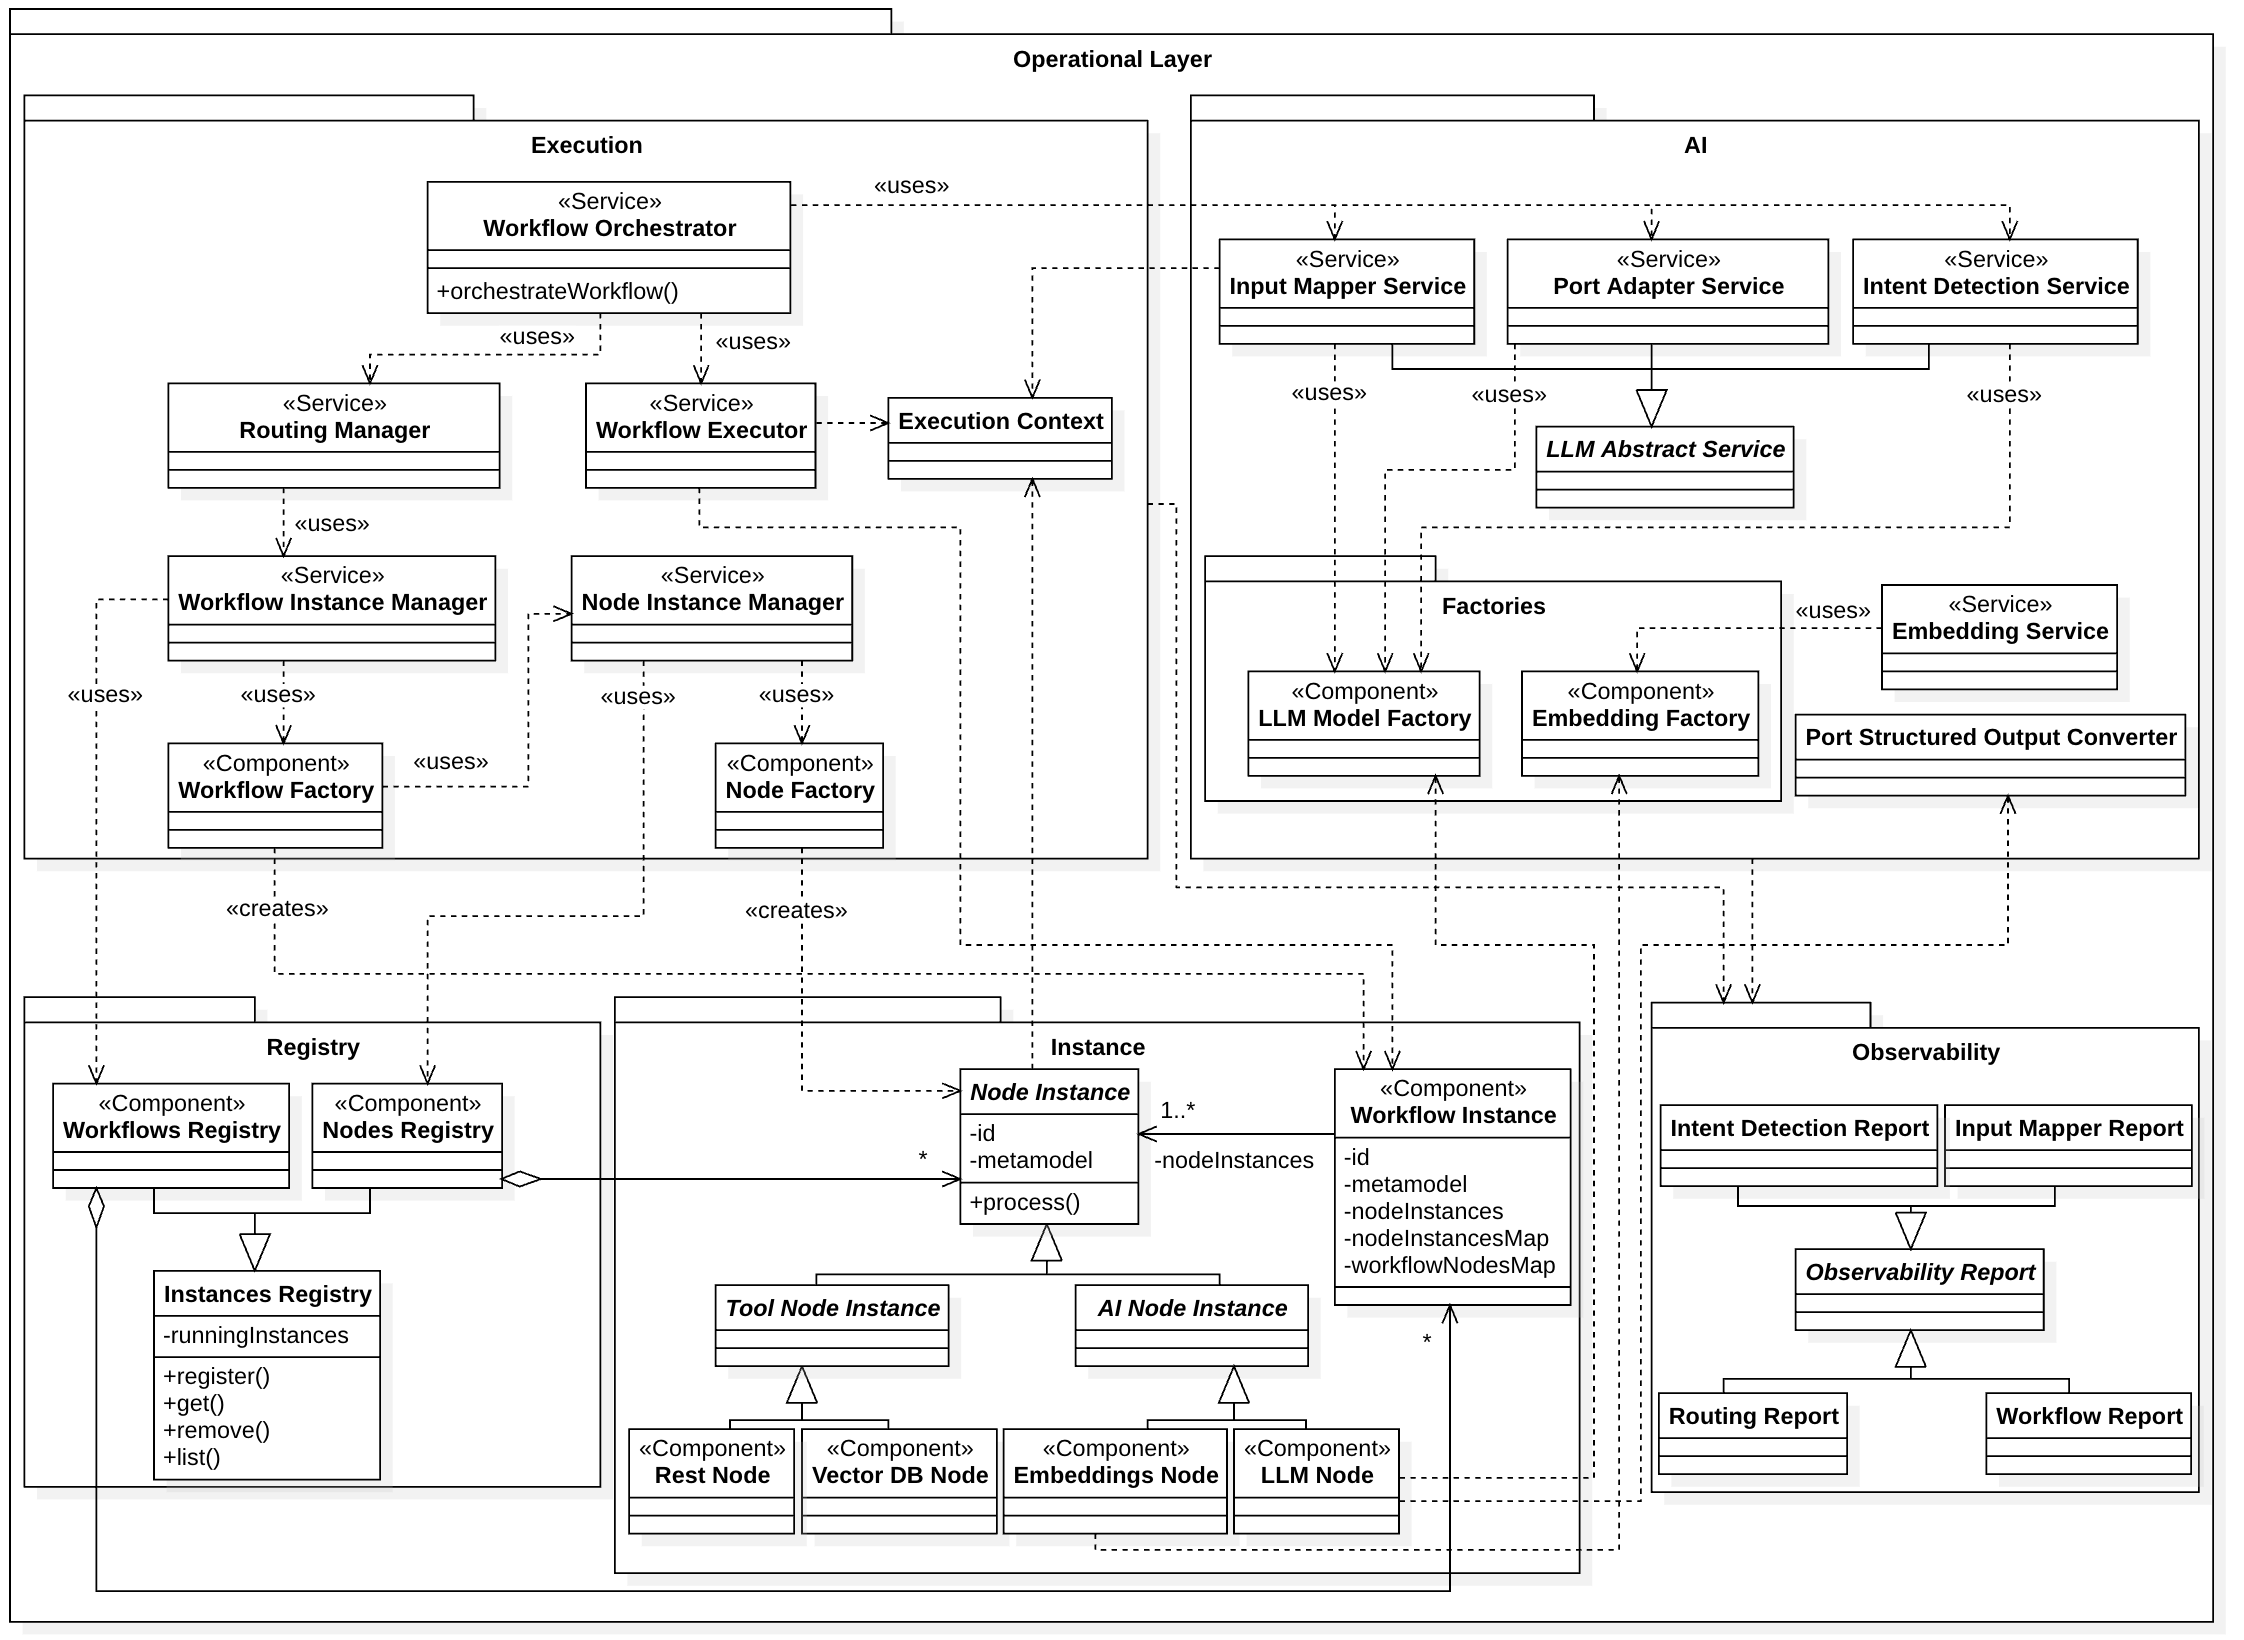
\includegraphics[width=1.2\textwidth]{Template_tesi/img/uml_operational.png}
  \end{adjustbox}
\caption{UML Diagram of the \texttt{Operational} package, presenting the core classes and their interactions within the operational layer. It details functionalities including workflow orchestration, AI services, instance management, and observability features. Standard getters/setters and non-essential elements are omitted for clarity.}
    \label{fig:uml_operational}
\end{figure}



Conversely, Figure~\ref{fig:uml_operational} illustrates the \textbf{Operational Layer}. This package includes the implementation of specialized workflow nodes that interact with external systems, such as databases, REST APIs, and AI service providers. Central to this layer is the \texttt{engine} package, which orchestrates the lifecycle of workflows—handling their retrieval, routing, and execution. Workflow and node instantiation are handled by specialized factory components, while two in-memory registries maintain records of active workflow and node instances, respectively. A significant component within the operational layer is the \texttt{AI} subpackage, which manages interactions with external providers of large language models and embedding services. It also exposes several essential LLM-powered services:

\begin{itemize}[leftmargin=*, label=--]
    \item \texttt{Input Mapper Service}: Translates user-provided request variables into the corresponding workflow inputs.
    
    \item \texttt{Port Adapter Service}: Resolves data-flow mismatches between workflow nodes.
    
    \item \texttt{Intent Detection Service}: Identifies and classifies the intent of the user.
\end{itemize}


\noindent
To enable dynamic and flexible model instantiation, a factory design pattern has been implemented. This allows LLM and embedding models to be initialized at runtime based on the specifications provided by the knowledge base. This approach encourages high configurability and supports seamless switching between different model providers, thus facilitating experimental evaluation and optimization.









\section*{AI Integration}

A central aspect of the system is the integration of large language models (LLMs) to enable cognitive workflows. For this purpose, Spring AI was selected as the primary framework (see Appendix \ref{ch:appendix_spring} for further details).
To evaluate both performance and system adaptability, multiple models and providers were tested across diverse services, demonstrating the flexibility offered by the model factories (see Figure \ref{fig:uml_operational}). Ultimately, \textbf{Claude 3.5 Sonnet} by Anthropic was selected for the \texttt{Input Mapper Service} and \texttt{Port Adaptation Service} due to its strong capabilities in schema handling, consistent structured outputs, and lower cost compared to more recent models like Claude 3.7 and Claude 4. For the \texttt{Intent Detector Service}, \textbf{GPT-4o} by OpenAI was integrated, providing state-of-the-art performance in intent classification. Finally, for generating embeddings, OpenAI’s \textbf{text-embedding-3-small} was employed to enable efficient vector search supporting intent classification.


\section*{Testing Summary}


The testing strategy covered unit, integration, and end-to-end tests, validating system correctness and robustness across 104 test cases:


\begin{itemize}[leftmargin=*, label=--]
    \item \textbf{Unit testing} involved 48 tests designed to verify the functionality of isolated components, such as metamodel validators and domain model methods.
    
    \item \textbf{Integration testing} included 54 tests that evaluated the interactions between components and services. LLM-based services were tested on real-world tasks spanning a wide range of scenarios, from simple to complex. Furthermore, the tests covered nodes that interact with external systems, such as database nodes and RESTful services, the latter simulated using WireMock\footnote{WireMock is an open-source tool for mocking HTTP-based APIs. See \url{https://wiremock.org}}.
    
    \item \textbf{End-to-end testing} involved two comprehensive tests simulating full workflow execution and adaptation in a production-like environment. These tests covered the entire process—from intent recognition to response generation—within the RAG scenario depicted in Figure~\ref{fig:RAG-workflow}.
\end{itemize}


A valuable insight from this testing regime is the role of integration tests that incorporate actual (non-mocked) LLM API calls. Although such tests incur considerable costs due to high API usage, they are essential for verifying system stability and functionality, particularly given the inherent non-deterministic nature of LLMs. By designing specific, nontrivial test cases that challenge the model's capabilities, this approach enables robust validation across different foundation models. It ensures resilience against potential regressions or failures resulting from model updates, optimizations, or changes in the underlying model provider.

It is important to note that, while database connections were mocked during the unit and integration testing phases to isolate system components, the end-to-end tests employed a dedicated MongoDB cluster. This environment was configured to closely replicate production conditions, providing a realistic scenario to validate the system's performance.


\subsection*{Test Coverage Report}
Table \ref{tab:code_coverage} presents the code coverage metrics of the implemented system.

\begin{table}[H]
\centering
\caption{Code coverage statistics by package.}
\label{tab:code_coverage}
\resizebox{\linewidth}{!}{%
\begin{tabular}{|l|c|c|c|}
\hline
\textbf{Package} & \textbf{Class Coverage} & \textbf{Method Coverage} & \textbf{Line Coverage} \\
\hline
\texttt{API} & 50\% (3/6) & 6\% (3/45) & 5\% (8/139) \\
\texttt{config} & 75\% (3/4) & 60\% (3/5) & 80\% (8/10) \\
\texttt{knowledge} & 88\% (55/62) & 73\% (244/333) & 63\% (902/1415) \\
\texttt{operational} & 77\% (51/66) & 71\% (236/332) & 75\% (1444/1906) \\

\hline
\textbf{Total (all packages)} & \textbf{80\% (112/139)} & \textbf{67\% (486/716)} & \textbf{68\% (2362/3471)} \\
\hline
\end{tabular}%
}
\end{table}






\section*{API Endpoints Overview}

The system exposes a RESTful API for manipulating the knowledge catalogs and performing requests. The following table summarizes the available endpoints, HTTP methods, and corresponding controllers.

\begin{table}[H]
\centering
\caption{Overview of exposed API endpoints and their respective controllers.}
\small
\begin{tabular}{|l|l|l|}
\hline
\textbf{Endpoint} & \textbf{Method} & \textbf{Controller} \\
\hline
\texttt{/api/workflows} & GET, POST & WorkflowController \\
\texttt{/api/workflows/execute} & POST & WorkflowController \\
\texttt{/api/workflows/\{id\}} & GET, PUT & WorkflowController \\
\hline
\texttt{/api/nodes} & GET, POST & NodeController \\
\texttt{/api/nodes/embeddings} & POST & NodeController \\
\texttt{/api/nodes/embeddings/\{id\}} & PUT & NodeController \\
\texttt{/api/nodes/gateway} & POST & NodeController \\
\texttt{/api/nodes/gateway/\{id\}} & PUT & NodeController \\
\texttt{/api/nodes/llm} & POST & NodeController \\
\texttt{/api/nodes/llm/\{id\}} & PUT & NodeController \\
\texttt{/api/nodes/rest-tool} & POST & NodeController \\
\texttt{/api/nodes/rest-tool/\{id\}} & PUT & NodeController \\
\texttt{/api/nodes/vector-db} & POST & NodeController \\
\texttt{/api/nodes/vector-db/\{id\}} & PUT & NodeController \\
\hline
\texttt{/api/intents} & GET, POST & IntentController \\
\texttt{/api/intents/\{id\}} & GET, PUT, DELETE & IntentController \\
\hline
\end{tabular}

\label{tab:api_endpoints}
\end{table}



\section*{Source Code Repository}
\noindent The complete source code is available at:
\begin{center}
\href{https://github.com/NiccoloCase/bsc-multi-agent-ai-framework}{\texttt{github.com/NiccoloCase/bsc-multi-agent-ai-framework}}
\end{center}

\noindent A permanent archive is accessible via DOI:
\begin{center}
\href{https://doi.org/10.5281/zenodo.15723912}{\texttt{doi.org/10.5281/zenodo.15723912}}
\end{center}

\noindent The repository contains all implementation files, documentation, and instructions necessary to reproduce the results described in this thesis.
\chapter{Comparative Analysis of LangChain and Spring AI
%LangChain and Spring AI
} \label{ch:appendix_spring}

This appendix presents a comparative analysis conducted to identify the most suitable framework for integrating large language models (LLMs) within the scope of this thesis project, ultimately motivating the decision to adopt a Java-based approach. The study focused on evaluating LangChain with Python and Spring AI with Java. The objective was to assess development experience, framework capabilities, and underlying design philosophies.



\section*{LangChain Overview}

LangChain is an open source framework introduced in October 2022, conceived to simplify the integration of LLMs into applications, allowing developers to build complex AI-powered systems. Over time, the LangChain ecosystem has grown to include additional tools such as LangGraph and LangSmith. Actively maintained by a passionate and growing community, LangChain has been widely adopted across various sectors, ranging from startups to large enterprises.
The framework is organized around modular components, such as chains, tools, memory, and agents, and offers seamless integration with a variety of foundational models, vector stores, APIs, and data loaders. LangChain also provides support for advanced agent architectures including \texttt{ReAct}, \texttt{MRKL}, \texttt{Plan-and-Execute}, and \texttt{BabyAGI}, enabling out-of-the-box capabilities for decision making and task decomposition.




\section*{Spring AI Overview}
Spring AI is an initiative within the Spring framework that facilitates the integration of generative AI capabilities into enterprise Java applications. Released in a milestone version in May 2024, its first stable release is expected by mid-2025\footnote{According to a recent update from the Spring team (April 2025), a release candidate (RC1) is scheduled for the following month, with a general availability (GA) release planned shortly after, in time for the Spring IO conference in Barcelona. See: \url{https://spring.io/blog/2025/04/10/spring-ai-1-0-0-m7-released} (accessed April 21, 2025).}. Some of the most notable features include:

\begin{itemize}[leftmargin=*, label=--] 
    \item \textbf{Spring Ecosystem Integration:} Seamlessly integrates with the existing Spring environment, enabling developers to leverage AI capabilities within the Spring ecosystem, following established Spring patterns.
    \item \textbf{Enterprise Scalability:} Designed to support enterprise-level applications, enabling the development of AI solutions that scale effectively in diverse environments. It provides robust scalability through its multi-threading capabilities and efficient use of the JVM, making Java preferable for handling complex concurrent workloads.
    \item \textbf{Seamless Deployment:} The Spring ecosystem provides a comprehensive framework that facilitates the efficient deployment of AI models in heterogeneous environments. Components such as Spring Boot and Spring Cloud support the scalable orchestration of microservices, making Spring particularly well-suited for production-ready, distributed AI systems.
\end{itemize}




\section*{Feature Comparison}


Spring AI and LangChain use distinct conceptual approaches. Among the key differences highlighted in Table \ref{tab:comparison}, the most notable is their support for agents, for which the two frameworks adopt fundamentally different strategies. LangChain follows an agent-first approach and natively supports several agent architectures, integrating a wide range of tools such as web search (allowing retrieval using the entire internet), databases, external APIs, and external applications. Conversely, Spring AI follows a more workflow-oriented approach, emphasizing \textit{Design for Reliability}. Drawing on insights from a research publication by Anthropic \cite{schluntz2024building}, it promotes simple, composable patterns rather than complex frameworks. At the time of writing, Spring AI does not directly integrate tools for creating agents. However, the Spring Blog \cite{tzolov2025agentic} documents \textit{Agentic Patterns} (e.g., Chain Workflow, Parallelization Workflow, Routing Workflow, and Orchestrator-Workers) that can be implemented using the framework. Consequently, there is currently no autonomous decision loop like LangChain's AgentExecutor or a native mechanism for automatic routing or re-planning (such as Plan-and-Execute). But this is likely to change as the project matures.


\begin{table}[htbp]
\caption{Comparison of Key Features Between LangChain and Spring AI for LLM-Based Application Development, updated as of April 2025}
\label{tab:comparison}
\begin{center}
\begin{tabularx}{\linewidth}{|l|X|X|}
\hline
\textbf{Feature} & \textbf{LangChain} & \textbf{Spring AI} \\ \hline
\textbf{Language Support} & Python—JavaScript and Java secondary & Java/Kotlin \\ \hline
\textbf{Design Approach} & Modular chains, tools, and memory components & Spring-style abstractions (e.g., templates, dependency injection) \\ \hline
\textbf{Model Providers} & 50+ supported providers & 15+ supported providers \\ \hline
\textbf{Agents} & Native support for agents and tools & Currently unsupported \\ \hline
\textbf{Vector Search} & Supported & Supported \\ \hline
\textbf{Web Search} & Supported (built-in APIs) & No native support; external integration required \\ \hline
\textbf{Web Scraping} & Supported (e.g., ScrapeGraph, WebVoyager, ScrapingAnt) & No native support; can be integrated externally \\ \hline
\textbf{State Management} & Conversation memory, LangGraph for workflows & Chat memory support \\ \hline
\textbf{Observability} & LangSmith integration for debugging and traces & Observability through Spring ecosystem tools \\ \hline
\textbf{Deployment} & Supports Docker/Kubernetes; flexible runtime environments & Optimized for Spring Boot and cloud-native deployments \\ \hline
\textbf{REST API Support} & Requires web frameworks like Flask, FastAPI, etc. & Built-in Spring Web support \\ \hline
\textbf{Primary Focus} & Rapid prototyping, research, startup-friendly & Enterprise-grade backend integration \\ \hline
\end{tabularx}
\end{center}
\end{table}




\section*{Development Experiment}

In order to assess the development experience with LangChain and Spring AI, two parallel Retrieval-Augmented Generation (RAG) pipelines were implemented, one in Python and the other in Java. The pipelines were developed using the following components:

\begin{itemize}[leftmargin=*, label=--] 
    \item \textbf{LangChain:} Utilized \texttt{FAISS} for similarity search and OpenAI \texttt{GPT-4}, served through \texttt{FastAPI}. 
    \item \textbf{Spring AI:} Employed \texttt{SimpleVectorStore} in-memory vector store, \texttt{GPT-4}, and exposed via REST APIs through \texttt{Spring Web}. 
\end{itemize}
    
The implementation of this comparative analysis is available in the corresponding GitHub repository\footnote{\url{https://github.com/NiccoloCase/bsc-multi-agent-ai-framework/tree/main/supplementary-materials/langchain-vs-springai}}. Please note that this project serves as a proof-of-concept to evaluate the development process and is not intended for production use.


\section*{Development Insights}

During the experimentation, several factors were taken into account, with the key differences summarized in Table \ref{tab:dev_results}.

A significant observation concerns the ease of setup, documentation, and community support for the two frameworks, which impact the overall development experience. Although LangChain provides extensive documentation, it can sometimes be fragmented and difficult to navigate—especially due to frequent updates that lead to outdated and conflicting information. Furthermore, the lack of clear overviews and guided introductions can leave beginners feeling overwhelmed. 
However, these issues are mitigated by an active community that consistently produces high-quality articles and resources. Additionally, LangChain is designed to be effortless to set up, especially with its straightforward installation process via \texttt{pip}. In contrast, Spring AI benefits from being part of the well-established Spring ecosystem. While the documentation is still evolving and on-line resources remain limited, its integration with Spring Initializr and its more focused scope make it easier for newcomers to get started. Furthermore, there is a reasonable expectation that Spring AI will adhere to the same principles of stability, backward compatibility, and enterprise-grade documentation of the Spring project.

Lastly, it is worth noting the relative verbosity of Java compared to Python, which can impact development speed, especially in tasks such as string manipulation and prompt construction. In this regard, Spring AI faces a disadvantage: operations that are concise in Python often require additional boilerplate in Java. This is especially evident in tasks like JSON parsing and construction. Spring AI addresses these challenges by offering higher-level abstractions, including helper classes like \texttt{PromptTemplate} and predefined prompt structures, which reduce manual string handling and streamline prompt creation. Nonetheless, Java's strong typing, robust IDE support, and mature build tools—such as Maven and Gradle—contribute to improved maintainability and reliability.

\begin{table}[htbp]
\caption{Development Experience: LangChain vs Spring AI}
\begin{center}
\renewcommand{\arraystretch}{1.2}
\begin{tabularx}{\linewidth}{|l|X|X|}
\hline
\textbf{Aspect} & \textbf{LangChain (Python)} & \textbf{Spring AI (Java)} \\
\hline
Ease of Setup & High & Moderate \\
\hline
Modularity & High & High \\
\hline
Integration with Backend & Low & High \\
\hline
Documentation  & Comprehensive & Growing \\
\hline
Community Support & Large and active & Emerging, backed by Spring ecosystem \\
\hline
\end{tabularx}
\label{tab:dev_results}
\end{center}
\end{table}




\section*{Conclusive Framework Choice and Motivation}

During the early design phase of this thesis, the choice between Java and Python was made. Python's extensive support for state-of-the-art LLM agents initially suggested it as the natural choice. However, Java's alignment with established software engineering principles—especially in terms of tooling, maintainability, and scalability—ultimately led to its preference. Its robust static typing system is particularly suited for implementing the reflective architecture proposed in this study: although type annotations were introduced in Python 3, Java's enforced type safety provides a more formal structural foundation for clearly demonstrating the Reflection Pattern. Furthermore, given that the project addresses themes such as Responsible AI and Software Transparency, Java's long-standing role in enterprise systems was a decisive factor. The inherent emphasis of the Spring ecosystem on scalability, security, and maintainability directly supports these objectives. Additionally, since the project was conceived to develop a structured meta-architecture for AI workflows from the ground up, advanced LangChain features—such as complex toolchains and built-in agentic patterns—were neither necessary nor aligned with the study's goals. Lastly, the novelty of Spring AI within the academic literature offered a valuable opportunity for original contribution.




\addcontentsline{toc}{chapter}{References}
\renewcommand{\bibname}{References}

\bibliographystyle{plain}
\bibliography{files/biblio}
\bibliographystyle{unsrt}
%\bibliography{sp,xml}

\end{document} 